\documentclass[
  fontsize=13pt,
  a4paper,
  chapterprefix,
    ]{scrbook}

\usepackage{emptypage}

\usepackage{geometry}
\geometry{a4paper,top=30mm,left=22mm,right=22mm,bottom=30mm,headsep=10mm,footskip=12mm}
\renewcommand{\baselinestretch}{1.05}\normalsize %Zeilenabstand
%vor Boston: 1.1 Zeilenabstand, Grösse 13 pt top=30mm,left=18mm,right=18mm,bottom=30mm,headsep=10mm,footskip=12mm

%distance between floats on the top or the bottom and the text, standard: 20.0pt plus 2.0pt minus 4.0pt
\setlength{\textfloatsep}{7pt plus 1.0pt minus 2.0pt}
% distance between two floats, standard: 12.0pt plus 2.0pt minus 2.0pt:
\setlength{\floatsep}{7pt plus 1.0pt minus 2.0pt}
%distance between floats inserted inside the page text (using h) and the text, standard: 12.0pt plus 2.0pt minus 2.0pt:
\setlength{\intextsep}{7pt plus 1.0pt minus 2.0pt}

\usepackage{indentfirst} %Einzug bei jedem Abschnitt

\usepackage{amsmath}
\usepackage{amssymb}
\usepackage{xfrac}

\usepackage[colorlinks = true,
            linkcolor = blue,
            urlcolor  = blue,
            citecolor = blue,
            anchorcolor = blue]{hyperref}
% must be after hyperref and amsmath
\usepackage[nameinlink]{cleveref}
  \crefname{figure}{FIG.}{FIGs.}
  \crefname{table}{TAB.}{TABs.}
  \crefname{equation}{EQ.}{EQs.}
  \crefname{section}{Section}{Section}

\usepackage{floatflt}
\usepackage{moresize}
\usepackage[]{ethimes}               % New styles and commands
\setcounter{tocdepth}{3} \setcounter{secnumdepth}{3}
\usepackage{fancyhdr}                % Headings
\usepackage{graphicx}                % EPS figures
  \graphicspath{
      {SECTION/30_Timeconstant/10_Figures/LaTeX/}
      {SECTION/30_Timeconstant/10_Figures/PGF/}
      {SECTION/30_Timeconstant/10_Figures/}
    }
\usepackage[dvips]{epsfig}           % EPS figures
\usepackage{epstopdf}
\usepackage{float}                   % Placement of floating objects
\usepackage{here}                   % Placement of floating objects
\usepackage{lipsum}                   %um eine Fussnote zu platzieren ohne Nr
\usepackage[ngerman, spanish, english]{babel}           %für Gänsefüsschen etc
\usepackage[utf8]{inputenc}\DeclareUnicodeCharacter{2212}{-}
\usepackage[T1]{fontenc}
\usepackage{siunitx} %SI units
    \DeclareSIUnit\samples{S} % frames per second
    \DeclareSIUnit\MS{\mega\samples\per\second} % frames per second
    % \DeclareSIUnit\Vrms{\volt_{rms}} % volt RMS
    \DeclareSIUnit\Vrms{V_{rms}} % volt RMS
    \DeclareSIUnit\fps{fps} % frames per second
\usepackage{rotating} % Rotating table
\usepackage{booktabs}
  \newcolumntype{x}[1]{>{\centering\arraybackslash\hspace{0pt}}p{#1}}
\usepackage{array}
\usepackage[table,xcdraw]{xcolor}

\usepackage{tabularx}

% \usepackage{cite}                    % bei Referenzen [15,12,11,10] sortiert es zu [10-12, 15]
\usepackage[
  backend=biber,
  hyperref,
  giveninits=true,
  doi=true,
  url=false,
    ]{biblatex}
\addbibresource{All.bib}
\addbibresource{supplemental.bib}
% \usepackage[square,numbers]{biblatex}
\usepackage{bm}

\newcommand\blfootnote[1]{%
  \begingroup
  \renewcommand\thefootnote{}\footnote{#1}%
  \addtocounter{footnote}{-1}%
  \endgroup
}

\usepackage[
  textformat=simple,
  labelfont=bf,
  format=hang]{caption}  %Caption options
\usepackage{afterpage}
\usepackage{subcaption}


\usepackage{fix-cm}
\usepackage{titlesec}
% \titleformat{\chapter}[display]
% {\bfseries\LARGE}
% {\vspace{-4ex}\selectfont\color{lightgray}\hfill
%   \Large\textrm{\chaptertitlename}
%   \fontsize{85}{70}\textbf{\thechapter}}
% {4ex}
% {}
% [\vspace{1ex}\titlerule]

\colorlet{chaptercolor}{blue!80!black}

\setkomafont{chapter}{\normalfont\color{chaptercolor}\huge}
\setkomafont{chapterprefix}{\Large}
\renewcommand*{\raggedchapter}{\raggedleft}
\renewcommand*{\chapterformat}{%
  \MakeUppercase{\chapappifchapterprefix{}}%
  \rlap{\enskip\resizebox{!}{1.2cm}{\thechapter} \rule{15cm}{1.2cm} }%
}
\RedeclareSectionCommand[beforeskip=30pt,afterskip=20pt]{chapter}
\renewcommand*\chapterheadmidvskip{\par\nobreak\vspace{10pt}}

\titleformat{\section}
{\normalfont\bfseries\Large}
{\thesection.}{0.5em}{}

\titleformat{\subsection}
{\normalfont\bfseries\normalsize}
{\thesubsection.}{0.5em}{}

\usepackage{fancyhdr}

\fancypagestyle{plain}{%
  \fancyhf{}%
  \fancyfoot[OR]{\textbf{\thepage}}%
  \renewcommand{\headrulewidth}{0pt}% Line at the header invisible
  \renewcommand{\footrulewidth}{0pt}% Line at the footer visible
}

\pagestyle{fancy}
\fancyfoot{}
\fancyhead{}
\renewcommand{\chaptermark}[1]{
  \markboth{\chaptername\ \thechapter.\ #1}{}}
\renewcommand{\sectionmark}[1]{
  \markright{\thesection.\ #1}}

\fancyhead[LE]{\bfseries\leftmark}
\fancyhead[RO]{\bfseries\rightmark}

\fancyfoot[LE,RO]{\textbf{\thepage}}
\renewcommand{\headrulewidth}{0.3pt}

\usepackage{tikz}
  \usetikzlibrary{external}
  \usetikzlibrary{
    calc,
    arrows,
    arrows.meta,
    shapes,
    positioning,
    decorations.markings,
    angles,
    intersections,
    matrix,
    fit,
    quotes,
    decorations.pathreplacing,%
    decorations.pathmorphing,%
    calligraphy,
    }

\tikzset{external/force remake}
\tikzset{external/system call={
  pdflatex \tikzexternalcheckshellescape -halt-on-error
  -interaction=batchmode -jobname "\image" "\texsource" && % or ;
  pdftops -eps "\image".pdf}}
  \tikzexternalize[prefix=Plots/cache/]
  % \tikzsetexternalprefix{Plots/Cache/}

\tikzset{>=latex}

\colorlet{colParticle}{black!10!}
\colorlet{colFluid}{blue!20!white}

\tikzset{
  fluid/.style = {
    fill=colFluid,
    fill opacity=.3,
    color=black,
  },
  particle/.style = {
    fill=colParticle,
    fill opacity=.3,
    color=black,
  },
  particleBall/.style = {ball color=colParticle},
}


\usepackage{pgfplots}
  % \usepgfplotslibrary{external}
  % \tikzexternalize
  \usepgfplotslibrary{groupplots}
  \usepgfplotslibrary{colormaps}
  % Define layers
  \pgfdeclarelayer{background}
  \pgfdeclarelayer{foreground}
  \pgfsetlayers{background,main,foreground}

\usepackage{tkz-euclide, tikz-cd}
\usepackage{tikz-3dplot}


\pgfplotsset{
  compat = 1.18,
  cycle list = {
    {black}, {lightgray},
    {black, densely dashed}, {lightgray, densely dashed},
    {black, dotted}, {lightgray, dotted},
    {black, loosely dotted}, {lightgray, loosely dotted}
  },
  width = 12cm,
  height = 9cm,
  every axis/.append style = {
    line width = 0.2mm,
    tick style = {line width = 0.2mm}
  },
  every axis plot/.append style = {
    line width = 0.4mm
  },
  enlarge x limits = false,
  enlarge y limits = {value = 0.05, auto},
  every axis legend/.append style = {
    nodes = right
  },
  xticklabel style={/pgf/number format/fixed},
  yticklabel style={/pgf/number format/fixed},
}

\makeatletter
\pgfplotsset{
/pgfplots/row step/.style={
/pgfplots/x filter/.append code={
        \ifnum\coordindex=0
                \def\c@pgfplots@eachnthpoint@xfilter{0}
                \edef\c@pgfplots@eachnthpoint@xfilter@cmp{#1}
        \else
                \pgfplotsutil@advancestringcounter\c@pgfplots@eachnthpoint@xfilter
                \ifx\c@pgfplots@eachnthpoint@xfilter@cmp\c@pgfplots@eachnthpoint@xfilter
                        \def\c@pgfplots@eachnthpoint@xfilter{0}
                \else
                        \let\pgfmathresult\pgfutil@empty
                \fi
        \fi
}
},
}
\makeatother
\pgfplotsset{filter discard warning=false}

 % Kapitel-Header-Stil
\newcommand{\relPath}{}
\newcommand{\cname}[1]{\citeauthor{#1}~\cite{#1}}
\newcommand{\cyear}[1]{In \citeyear{#1}, \cname{#1}}

\def\svginput{\input}

\newcommand{\figWidth}{80mm}
\newcommand{\figWidthDouble}{160mm}
\newcommand{\subfigWidth}{75mm}


\newcommand{\tikzHelper}{a}
\newcommand{\tmp}{a}

\newcommand{\SiO}{SiO$_{2}$}

\newcommand{\comsol}[1]{({\ttfamily #1})}

\newcommand{\conj}[1]{#1^{\ast}}

\newcommand{\pertubationorder}[2]{
  #1^{(#2)}
}

\newcommand{\zeOrder}[1]{
  \pertubationorder{#1}{0}
}

\newcommand{\stOrder}[1]{
  \pertubationorder{#1}{1}
}

\newcommand{\ndOrder}[1]{
  \pertubationorder{#1}{2}
}

\newcommand{\MR}[1]{\mathrm{#1}}

\newcommand{\bessel}[2]{j_{#1}\left(#2\right)}
\newcommand{\dbessel}[2]{j^{\prime}_{#1}\left(#2\right)}
\newcommand{\hankel}[2]{h_{#1}\left(#2\right)}
\newcommand{\dhankel}[2]{h^{\prime}_{#1}\left(#2\right)}
\newcommand{\legendre}[2]{P_{#1}\left(#2\right)}

\newcommand{\xv}{x_{\MR{v}}}

%%%%%%%%%%%%%%%%%%%%
%%%% MATH Commands
%%%%%%%%%%%%%%%%%%%%
\newcommand{\stress}{\sigma_{ij}}
\newcommand{\stresstensor}{\bm{\underline{\underline{\sigma}}}}

\newcommand{\intensity}{I}

\newcommand{\wavenumber}{k}
\newcommand{\wavevector}{\vb{\wavenumber}}

\newcommand{\fresnelR}{\mathcal{R}}
\newcommand{\fresnelT}{\mathcal{T}}
\newcommand{\fresnelr}{r}
\newcommand{\fresnelt}{t}

\newcommand{\cNA}{C_{\MR{NA}}}

\newcommand{\incident}{\theta_{\MR{i}}}
\newcommand{\reflected}{\theta_{\MR{r}}}
\newcommand{\transmitted}{\theta_{\MR{t}}}

\newcommand{\lbeta}{\beta}

\newcommand{\vbl}{\delta}

\newcommand{\normalized}[1]{\tilde{#1}}

\newcommand{\refraction}{n}

\newcommand{\nf}{\refraction_{\MR{f}}}
\newcommand{\ns}{\refraction_{\MR{s}}}


\newcommand{\normal}{n_{i}}
\newcommand{\normalvector}{\vb{n}}

\newcommand{\speed}{c}

\newcommand{\pre}{p}
\newcommand{\velpotential}{\phi}

\newcommand{\vel}{v}
\newcommand{\velvector}{\vb{\vel}}

\newcommand{\power}[2]{P_{\MR{#1}}^{(#2)}}

\newcommand{\timeaverage}[1]{\left\langle #1 \right\rangle}

\newcommand{\force}{F}
\newcommand{\forcevector}{\vb{\force}}

\newcommand{\FARF}{\forcevector^{\MR{rad}}}
\newcommand{\FAS}{\forcevector^{\MR{drag}}}

\newcommand{\DV}{\Delta V}
\newcommand{\Dx}{\Delta x}
\newcommand{\Dy}{\Delta y}
\newcommand{\Dz}{\Delta z}

\newcommand{\fs}{f_{\MR{s}}}

\newcommand{\Dfour}{\SI{4.39}{\micro\meter}}
\newcommand{\Dtwo}{\SI{2.06}{\micro\meter}}
\newcommand{\R}{R}
\newcommand{\Rprime}{R^{\prime}}
\newcommand{\Rtwo}{R_{2}}
\newcommand{\Rfour}{R_{4}}

\newcommand{\RA}{R_{\MR{QPD}}}

\newcommand{\Dt}{\Delta t}

\newcommand{\ex}{\vb{e}_{x}}
\newcommand{\ey}{\vb{e}_{y}}
\newcommand{\ez}{\vb{e}_{z}}

\newcommand{\fex}{f_{\MR{ex}}}

\newcommand{\wavelength}{\lambda}

\newcommand{\lap}{\wavelength_{\MR{p}}}
\newcommand{\laF}{\wavelength_{\MR{F}}}
\newcommand{\lal}{\wavelength_{\MR{l}}}

\newcommand{\viscosity}{\mu}
\newcommand{\density}{\rho}
\newcommand{\kinematicviscosity}{\nu}

% fluid properties
\newcommand{\cfl}{c_{\MR{f}}}
\newcommand{\muef}{\viscosity_{\MR{f}}}
\newcommand{\rhof}{\density_{\MR{f}}}

\newcommand{\rhop}{\density_{\MR{p}}}

\newcommand{\timeconstant}[1]{\tau_{\MR{#1}}}

\newcommand{\tdrag}{\timeconstant{drag}}
\newcommand{\tOT}{\timeconstant{OT}}
\newcommand{\tas}{\timeconstant{AS}}
\newcommand{\tarf}{\timeconstant{ARF}}
\newcommand{\tqpd}{\timeconstant{QPD}}
\newcommand{\tiner}{\timeconstant{iner}}

% nomarlized measures
\newcommand{\tkappa}{\tilde{\kappa}}
\newcommand{\trho}{\tilde{\rho}}
\newcommand{\tdelta}{\tilde{\delta}}
% imaginary unit
\newcommand{\iu}{\MR{i}\mkern1mu}

\newcommand{\um}{\si{\micro\meter}}
\newcommand{\rpm}{rpm}

\newcommand{\normBdLayer}{\tilde{\delta}}
\newcommand{\finalOmega}{\Omega_{\MR{equ}}}

\newcommand{\Rcrit}{\R_{\mathrm{crit}}}
\newcommand{\fp}{f_{\mathrm{p}}}
\newcommand{\cf}{\cfl}
% nomarlized measures
\newcommand{\llaser}{\lal}
 % Kapitel-Header-Stil

\renewcommand{\\}{\par}
%damit wird jeder Abschnitt zum Paragraph, wodurch man unten mittels
%\setlength{\parindent}{5mm} einen Einzug definieren kann nach jedem "\\"

\begin{document}

\hyphenation{ acou-sto-pho-re-sis re-so-na-tors wave-length quar-ter}
\pagenumbering{roman}
\pagestyle{fancy}                   % Special headings

\setlength{\parindent}{4mm}       % Paragraph Einzug am Anfang jedes Paragraphen

\begin{titlepage}
  {Diss. ETH No. tbd. (1c41d78) \vspace{2.5cm}}
\begin{center}
\Large{\textbf{Experimental Validation of\\ Acoustofluidic Theory and 
Simulations\\ using an Optical Trapping Set-Up}}
\end{center}
\vspace{2.0cm}
\begin{center}
{A thesis submitted to attain the degree of}
\end{center}
\begin{center}
{\textsc{Doctor of Sciences of ETH Zurich}}\\
%{SWISS FEDERAL INSTITUTE OF TECHNOLOGY ZURICH}
{(Dr. sc. ETH Zurich)}
\end{center}
\vspace{10mm}
\begin{center}
{presented by}
\end{center}
\begin{center}
  {\textsc{\underline{Christoph} Ludwig Georg Ananda Goering}}
\end{center}
\begin{center}
%{MSc\ ETH \ ME \\
{M.Sc. in mechanical engineering from\\
Technische Universit\"at M\"unchen,\\
born on 17$^{\text{th}}$ August 1991,\\
citizen of Germany.}
\end{center}
\vspace{10mm}
\begin{center}
{accepted on the recommendation of \\ \vspace{0.3cm}
Prof.\ Dr. J\"urg Dual, examiner \\
Prof.\ Dr. Daniel Ahmed, co-examiner}
\end{center}
\vspace{5mm}
\begin{center}
2022
\end{center}

\cleardoublepage
\thispagestyle{empty}
\vspace*{5.0cm}

\begin{flushright}
% \begin{center}
\vspace*{0.5cm}
\large
\textit{Die Berge sind nur so schön,\\ weil Täler dazwischen liegen.}
% \vspace*{0.5cm}
% Albert Einstein\\
% \vspace*{2cm}

% Ich widme diese Dissertation \\
% meinen Eltern Heike und Klaus sowie meiner Verlobten Rebecca,\\
% \end{center}
\end{flushright}

\clearpage
\cleardoublepage
\end{titlepage}

\chapter*{Preface}
I would like to express my deepest gratitude for the opportunity to conduct my 
doctoral studies in the group of Mechanics and Experimental Dynamics, Institute 
for Mechanical Systems, Department of Mechanical and Process Engineering, ETH 
Zurich in the years 2016-2021. During these five years, I had the opportunity 
to acquire a diverse skill set and pursue interdisciplinary research projects, 
which would not have been successful without the tremendous support from my 
colleagues, project partners and supervisor. I would like to thank everyone who 
helped me in these five fantastic, diverse and intense years. Following, I 
would like to highlight some persons who deserve to be mentioned by name:

\begin{itemize}

\item First of all, I would like to express my deepest gratitude to Jürg Dual. 
  Despite his hands-off supervision style, which enabled me to develop my full 
  potential, I could always count on his support and corrections in my 
  ambitions to save me from gross mistakes. Jürg is one of the best supervisors 
  I had the pleasure to get to know and one of my idols with regards to 
  interpersonal competences and my future academic career.

\item I would like to thank Thomas Laurell for accepting to co-examine my 
  dissertation and for various meetings that increased the quality of my 
  publications and gave me indispensable ideas for my future academic career.

\item Special thanks go to Thierry Baasch. Thierry not only always had an 
  answer to all work related questions but also an open ear for things that did 
  not necessarily relate to my doctoral studies. He is a great mentor and 
  friend.

\item I would also like to especially thank Nino Läubli who was the driving 
  force behind our two collaborations that we managed to render successful 
  within a short amount of time. Despite his tight schedule, Nino always took 
  the time to help me on various occasions, especially regarding paper 
  optimisation and revision.

\item Without my first project partner, Dominik Haidas, who supported me in 
  droplet microfluidics and project management related questions, I would not 
  have been able to develop skills in this area, which are indispensable for my 
  future career.

\item My special gratitude also goes to Peter Ruppen. Without Peter, one of my 
  best device ideas would have ended unnoticed inside a cupboard. With his 
  expertise in bacteria handling, we were able to transform a previously 
  unnoticed device design into a patent and publication.

\item I would like to thank my collaborators from the "Powder Focusing" 
  project: Patrik Rohner, Shahab Eghbali, Choi Kwanghoon, and S\'ebastien 
  Vaucher for the refreshing and fruitful meetings.

\item I would like to thank everyone that I had the pleasure of getting to know 
  during various conferences and inspired me on various occasions, particularly 
  the ones from our acoustofluidics community. Especially, I would like to 
  thank Rune Barnkob, who is one of my role models regarding sophisticated 
  research and being a great mentor.

\item I would like to thank the operation team of the BRNC cleanroom for the 
  help with various chrome masks and device production. Especially, I would 
  like to thank Ute Drechsler. Ute is one of the most proficient persons 
  regarding clean room production I have ever met. With her limitless effort, 
  she manages to support all cleanroom users within their projects, keeps the 
  machines in BRNC up and running, and pursues her own projects for IBM, 
  simultaneously. Ute is one of my role models regarding dedication and passion 
  for her work.

\item The help regarding administrative tasks from Beate Fonf\'e, clean room 
  fabrication from Donat Scheiwiler and Stafan Blunier, small adjustments with 
  high impact at my experimental setups form Jean-Claude Thomasina, and 
  electronic equipment form Bernhard Zybach layed the basis for the success of 
  my experimental work. Thank you very much Beate, Donat, Stefan, Jean-Claude, 
  and Bernhard!

\item I would like to thank Anja Huss from Thorlabs GmbH. Together with here 
  competent support, we have been able to design three highly personalised 
  experimental setups, essential for the success of all presented projects in 
  this thesis.

\item I would like to thank my colleagues in the group of Mechanics and 
  Experimental Dynamic, Ivo Leibacher, Peter Reichert, Tobias Brack, Valentin 
  van Gemmeren, Dhananjay Deshmukh, Christoph Goering, Jonas Fankhauser, Cooper 
  Harshbarger and Alen Pavlic for their continuous support.

\item I would like to thank all students that I had the pleasure to supervise. 
  Without your work, I would not have been able to pursue so many ideas 
  simultaneously. Especially, I would like to thank Aurelia Bucciarelli, Marco 
  Hoseneder, Moritz Leuthner, Michel Manser, Alexandre Ratschat and Philipp 
  Suter who contributed significantly to my publications.

\item Last but not least, I would like to thank my family and friends, who 
  rendered the time during my doctoral studies even more enjoyable.

\end{itemize}

Even though doctoral theses tend to be forgotten after some years, I hope that 
I could make a significant contribution in the research area of acosutofluidics 
and show that there is still plenty of room for further improvements. My 
deepest desire is to use my knowledge for the development of novel applications 
that can tackle the great challenges that our generation has to face.

\begin{flushleft}
\begin{figure}[h]
\begin{flushleft}
 \hspace{1 cm}
 
\includegraphics[height=3cm]{Unterschrift.png}
\end{flushleft}
\end{figure}
\vspace{-0.1 cm}
\hspace{1 cm} Christoph Goering\\
\hspace{1 cm} Baar, May 2022
\end{flushleft}


\tableofcontents

\cleardoublepage
\pagenumbering{arabic}
\chapter*{Abstract} \markboth{Abstract}{Abstract}
\addcontentsline{toc}{chapter}{Abstract}
%Abstract structure: background – activity/purpose – methods – results – 
%conclusion (BAMRC)

A typical channel within a micro-scale acoustofluidic (MSAF) device has a small 
cross-section where the height is usually less than \SI{200}{\um} and the width 
less than \SI{5}{\mm}; the length can be up to several \si{\cm}, however, often 
is not of big interest. Direct measurement of, e.g., the pressure produced by 
the acoustic excitation is impossible due to the smallness of the region of 
interest. Additionally, the acoustic driving frequencies are generally above 
\SI{100}{\kilo\hertz} such that the time resolution of measurements must be 
even at least twice as high if one is also interested in the transient 
behaviour and build up of, e.g., the acoustic pressure field and not only the 
steady-state.

At the moment, the most common and straightforward way to approximate the 
acoustic pressure within the channel is to optically measure the velocity of 
several objects of known size and material properties and then calculate back 
which pressure would have led to this velocity. The validity and correctness of 
the pressure approximation depends on several uncertainties. Besides the object 
dimensions and the material parameters of the object and the fluid, the biggest 
uncertainty is the validity of the underlying theory of the acoustic radiation 
force (ARF) that is used for the calculation. There exist many MSAF models for the 
calculation of the acoustic forces which differ mainly in the assumptions 
regarding the physical model for the fluid and the immersed object. Each theory 
has its parameter space where it is superior to the others because it includes, 
e.g., the effect of visco-elasticity of the fluid.

Here, an optical trapping (OT) apparatus is utilized to investigate two 
phenomena where controversies exist in the MSAF community: 1) the transient 
build up of the ARF and the drag force from acoustic streaming (AS) for a 
continuous and pulsed acoustic excitation; 2) the quantification of the 
steady-state rotational velocity of a spherical particle driven by the acoustic 
viscous torque where the viscous boundary layer (VBL) thickness is comparable 
to the particle radius itself.

So far, OTs have mainly been used as force sensors on single particles within 
MSAF devices. For the measurements of both phenomena we take advantage of the 
fine spatial and temporal resolution that the OT offers, as well as the OT 
property that single particle measurements are possible.

In order to measure the build up of the ARF and AS, an acoustic excitation 
frequency and measurement location within the standing pressure wave was used 
where the two forces were orthogonal to each other. The orthogonality as well 
as the division into ARF and drag force from AS was measured and validated by 
force measurements with the OT throughout the fluid channel with differently 
sized particles.

The results of a continuous excitation showed that the ARF starts to build up 
almost instantaneously after the acoustic excitation was switched on, whereas 
the AS takes significantly longer. Interestingly, the fast ARF build up was 
expected from theoretical considerations, but the slow AS build up was 
underestimated by a factor of about 4. The pulsed excitation experiments 
revealed that depending on the specific pulse parameters the build up of AS can 
be suppressed substantially while the ARF is not affected as much as AS. 
Therefore, smaller particles can still be mainly manipulated by the ARF because 
the relative importance of AS decreases for a pulsed excitation faster than for 
the ARF. Our measurements strengthen experimental findings for a pulsed 
excitation that could not yet be explained theoretically.

For the steady-state rotational speed measurement, a high viscosity mixture of 
water with glycerol (7 to 3) was created such that the formed VBL around the 
particle was about the same as the particle radius. The phase difference 
between two acoustic excitation sources spatially orthogonal to each other led 
to a time-averaged acoustic streaming field in the VBL of the particle along 
its circumference. This streaming field creates a driving viscous torque that 
causes a rotation with the rotational velocity at which the driving viscous 
torque equals the counteracting viscous drag torque.

A theoretical formula overestimates the steady-state rotational speed for the 
experimental parameters by more than one order of magnitude. This was expected 
because, up to now, there are no theories that are valid for the regime where 
the radius is the same size as the VBL. However, a numerical study investigated 
exactly this regime and proposed a calculation for the final rotational 
velocity including the effects of the VBL. The rotational velocities measured 
with the OT confirmed two points: 1) the expected invalidity of the simplified 
theory in the regime of high viscosity and, hence, the necessity of its 
inclusion in the calculations; 2) the correctness of the numerical results.


\chapter*{Zusammenfassung}
\markboth{Zusammenfassung}{Zusammenfassung}
\addcontentsline{toc}{chapter}{Zusammenfassung}

Die typischen Dimensionen eines Flüssigkeitskanals für eine micro-scale 
acoustofluidic (MSAF) Anwendung ist eine Höhe von weniger als \SI{200}{\um}, 
eine Breite von weniger als \SI{5}{\mm} und einer Länge von mehreren \si{\cm}, 
wobei die Länge nicht von grosser Wichtigkeit ist. Die direkte Messung von 
physikalischen Grössen, wie zum Beispiel, dem Druck generiert durch die 
akustische Anregung ist unmöglich, da der Bereich der Messung klein ist.  
Ausserdem sind die akustischen Frequenzen generell grösser als 
\SI{100}{\kilo\hertz}, so dass die Messfrequenz mindestens doppelt so hoch sein 
muss, wenn unter anderem auch das transiente Verhalten and der Aufbau des 
akustischen Drucks von Interesse ist und nicht nur dessen eingeschwunger 
Zustand.

Bis jetzt ist die häufigste und einfachste Methode den akustichen Druck 
innerhalb der Fluidkanals abzuschätzen, die Geschwindigkeiten von mehreren 
Objekten mit bekannten Dimensionen and Materialparameteren optisch zu messen 
und dann anhand der Geschwindigkeiten auf den herrschenden aktustischen Druck 
zurückzurechnen. Die Validität und Richtigkeit der Druckabschätzung hängt von 
mehreren Unsicherheiten ab. Neben den Dimensionen des Objekts und den 
Materialparameteren des selbigen und des Fluids die grösste Unsicherheit ist 
die Validität der angewendeten Theorie für die Berechnung der \emph{acoustic 
radiation force (ARF)}. Es gibt viele Model für MSAF, welche die akustischen 
Kräfte herleiten und berechnen.  Sie unterscheiden sich grösstenteils bei der 
Annahme des physikalischen Models für das Objekt und das Fluid. Jede Theorie 
für sich hat einen Parameterbereich, wo sie genauer ist als die anderen, weil 
sie zum Beispiel die Viskoelastizität des Fluids berücksichtigt.

In dieser Arbeit wird eine optische Falle (oF) verwendet, um zwei MSAF 
Phänomene zu untersuchen, bei welchen es ungeklärte Kontroversen gibt: 1) der 
transiente Aufbau der ARF und der \emph{drag force from acoustic streaming 
(AS)} für eine ununterbrochene und eine gepulste akustische Anregung; 2) die 
Quantifizierung der stationären Rotationsgeschwindigkeit eines spährischen 
Partikels, welches durch den \emph{acoustic viscous torque} angetrieben wird 
und welches eine \emph{viscous boundary layer thickness} (VBL) hat, die so 
gross wie der Partikelradius selbst ist.

Bisher sind oFn vor allem als Kraftsensoren für einzelne Partikel innerhalb von 
MSAF Geräten eingesetzt worden. Für die Messung der genannten Phänomene nutzen 
wir die genaue örtliche und zeitliche Auflösung der oF aus, wie auch die 
Möglichkeit Messungen an einzelnen Partikeln durchzuführen.

Für die Messung des Aufbaus der ARF und des AS wurde eine akustische 
Anregungfrequenz und Messpunkte innerhalb der stehenden Druckwelle verwendet, 
bei deren Kombination die ARF and die Kräfte von AS senkrecht zueinander waren.  
Die Rechtwinkligkeit als auch die Aufteilung in ARF und AS wurde durch mehrere 
Kraftmessungen innerhalb des ganzen Fluidkanals mit unterschiedlichen 
Partikelgrössen validiert.

Die Ergebnisse der ununterbrochenen Anregung zeigten, dass der Aufbau der ARF 
sofort nach Beginn der aktustischen Anregung beginnt, wohingegen AS deutlich 
langsamer ist. Der zügige Aufbau der ARF wird von der Theorie in der 
Geschwindigkeit vorhergesagt, wobei der Aufbau des AS um den Faktor 4 
unterschätzt wird. Die Experimente mit einer gepulsten Anregung zeigten, dass 
abhängig von den Pulsparametern der Aufbau von AS weitesgehend verhindert 
werden kann, aber der Aufbau der ARF nicht im gleichen Masse beeiträchtigt 
wird. Daher werden kleinere Partikel zum grössten Teil wegen der ARF 
manipuliert, weil die relative Wichtigkeit von AS für eine gepulste Anregung 
schrumpft. Unsere Experimente bestärken die andere experimentelle Ergebnisse 
mit einer gepulsten Anregung, welche bisher durch keine Theorie erklärt werden 
können.

Für die Messung der stationären Rotationsgeschwindigkeit wurde eine Mischung 
zwischen Wasser und Glycerol (7 zu 3) hergestellt, dessen Viskosität so gross 
war, dass die VBL um das Partikel herum in etwa so gross wie der Partikelradius 
selbst war. Die Phasenverschiebung zwischen der beiden aktustischen Anregung 
die räumlich senkrecht zueinander standen führte zu einem zeitgemittelten AS 
Feld innderhalb der VBL in Richtung des Äquators des Partikels. Dieses AS Feld 
ist der Ursprung für ein antreibendes akustisch viskoses Drehmoment, welches 
das Partikel bis zu der Rotationsgeschwindigkeit beschleunigt, wo das 
Antriebsmoment das gegengerichtete viskose Widerstandsmoment gleicht.

Eine theoretische Formel überschätzt die stationäre Rotationsgeschwindigkeit 
für die experimentellen Parameter mit mehr als einer Grössenordnung. Dieser 
Fehler war erwartete, weil es bis jetzt noch keine Theorie gibt, welche für den 
Fall gilt, wo der Partikelradius so gross ist wie die VBL selbst. Eine 
numerische Studie untersuchte unter anderem diesen Parameterbereich für 
spährische Partikel und gab eine Formel für die stationäre 
Rotationsgeschwindigkeit an, welche die viskosen Effekte der VBL 
berücksichtigt. Die mit der oF gemessenen Rotationsgeschwindigkeiten 
bestätigten zwei Punkte: 1) die erwartete Üngültigkeit der vereinfachten 
Theorie für hohe Viskositäten und daher die notwendige Berücksichtigung der 
Viskosität; 2) die Richtigkeit der numerischen Ergebnisse.


\cleardoublepage
\renewcommand{\relPath}{SECTION/30_Timeconstant}
 
\chapter[Dynamic Timeconstant Measurement]{Dynamic Measurement of the Acoustic 
Streaming Time Constant utilizing an Optical Tweezer}\label{ch:timeconstatn}
\textit{This chapter resulted from a collaboration between the Bioanalytics 
  Group, Department of Biosystems Science and Engineering, ETH Zurich, Basel, 
  and the Mechanics and Experimental Dynamics group, Department of Mechanical 
  and Process Engineering, ETH Zurich, Zurich. We successfully combined the 
  expertise of both groups, namely droplet microfluidics and cell culturing 
  (Dominik Haidas), and acoustic particle manipulation (Michael Gerlt). The 
  chapter has been published previously in the journal Biomicrofluidics:
\footnote{: DOI: 10.1103/PhysRevE.104.025104, reproduced with permission, 
copyright 2020 AIP Publishing.}}

\vspace{5mm} \noindent
C. Goering and J. Dual, "Dynamic measurement of the acoustic streaming time 
constant utilizing an optical tweezer", Physical Review E, 2021, \textbf{104}, 
025104.


\section{Abstract}
Two orthogonal standing acoustic waves, generated by piezoelectric excitation, 
can form a two-dimensional pressure field in microfluidic devices. A phase 
difference of the excitation waves can be employed to rotate spherical 
\si{\micro\meter}-sized silica particles by a torque mediated through the 
viscous boundary $\delta$ around the particle.

The measurement of the rotational rate is, so far, limited to high-speed cameras 
and their frame rate, and gets increasingly difficult when the sphere gets 
smaller.  We report here a new method for measuring the rotational rate of 
\si{\micro\meter} sized spherical particles. We utilize an optical trap with 
high-speed position detection to overcome the frame rate limitation of wide 
field image recording. The power spectrum of an optically trapped, rotating 
particle reveals additional peaks corresponding to the rotational frequencies -- 
compared to a non-rotating particle. We validate our method at low rotational 
rates against high-speed video observation. 

To demonstrate the potential of this method we addressed a recent controversy 
about the rotation of particles with a relatively large VBL 
$\delta$. We measured steady-state rotational rates up to \SI{229}{\hertz} 
(\SI{13.8e3}{\rpm}) for a particle with a radius $R \approx \delta$.  Recent 
numerical research suggests that in this regime the existing theoretical 
approach (valid for $R\gg\delta$) overpredicts the steady-state rotational rate 
by a factor of 10.  With our new method we also confirm the numerical results 
experimentally.

\section{Introduction\label{sec:TC-introduction}}

In recent years, acoustofluidics has provided many powerful tools. Due to being 
contact-less, label-free, and biocompatible 
\cite{Antfolk2015,Abdulla2020,Zielke2020,Binkley2020,Cai2020}, acoustofluidic 
manipulation can be used in medical applications for cancer research
\cite{Antfolk2015,Abdulla2020,Zielke2020,Binkley2020}, Alzheimer research 
\cite{Cai2020}, targeted drug delivery \cite{Bose2015}, and for pumping medical 
fluids \cite{Wu2019}. In addition, there are biological 
\cite{Gerlt2020,Xie2019} and engineering applications (e.g., micro-pumping 
\cite{Wu2019,Huang2014,Lin2019,Ozcelik2021}).

Most of these applications utilize the acoustic radiation force (ARF) to 
manipulate objects on the micro-scale. The ARF is a second-order time-averaged 
effect that arises from the interaction of an acoustic field scattered at an 
object surface and a background acoustic field 
\cite{Doinikov1994Rigid,Hasegawa1969,Yosioka1955,Gorkov1962,Bruus2012}.
These objects can be solid particles, air bubbles, fluid droplets, biological 
samples, as long as their material properties (density $\rho$ and speed of 
sound $c$) are different from the surrounding medium. However, there coexists 
a fluid motion called acoustic streaming (AS) 
\cite{Nyborg1965,Kolb1956,Nyborg1953}. This motion can arise either from
viscous losses in the fluid (Eckhart type streaming \cite{Eckart1948}) or it 
can arise in the viscous boundary layer at a fluid to wall interface 
(Schlichting and Rayleigh streaming \cite{Riley1998,Schlichting1932}).


The theoretical derivations usually describe the steady-state of the AS field. 
A theoretical numerical study \cite{Muller2015} investigated the temporal build 
up of the ARF and AS field. In contrast to the ARF, the viscous drag force 
arising from AS is independent of the object material properties because it is 
a motion of the fluid. The AS direction coincides with the direction of the 
relative motion between fluid and particle.

For a spherical object of radius $R$, the drag force in laminar flow scales 
linearly with the object radius $\FAS \propto R$. In contrast to the $\FAS$, 
the ARF scales with the volume $\FARF \propto \R^{3}$ \cite{Bruus2012-10}.  
Based on the fluid and the object material properties, the $\FARF$ will 
dominate over the $\FAS$ if the radius $\R$ is greater than the critical radius 
$\R_{\text{crit}}$, where $\FAS = \FARF$ holds. The direction of $\FAS$ can be 
different from the $\FARF$. Therefore, the $\FAS$ is usually undesired.

The ARF and the AS occur not only in the bulk of the fluid, but also on sharp 
edges of a device \cite{Doinikov2020a,Doinikov2020b,Leibacher2015,Nama2016}. 
So-called micro-streaming around the surface of a spherical particle can even 
cause a sign inversion of the ARF if the viscous boundary layer $\delta$ is 
sufficiently large \cite{Baasch2019}. However, there are applications that take 
advantage of the AS \cite{Antfolk2014,Mao2017,Hao2020}: a complete overview of 
AS applications can be found in \cite{Wiklund2012a}.

In literature, it is well understood how long it takes until the acoustic 
field, and hence the ARF, needs to build up \cite{Muller2015} and how long the 
particle focusing takes \cite{Bruus2012-10}. However, it is still not fully 
clear how long it takes for the AS to build up, and what the definition for the 
analytical AS time constant is. In the acoustofluidics community, it is 
generally accepted that the build up for the AS field takes longer than the 
build up of the ARF. By using a pulsed actuation of the acoustic field and 
therefore exploiting this time offset, \citeauthor{Hoyos2013} prevented the 
build up of AS \cite{Hoyos2013,Castro2016}. They varied the number of periods 
for which the acoustic actuation is switched on and off, respectively. They 
experimentally showed that for a ratio of about 1 to 1 between 500 on- and 500 
off-periods the streaming velocity is less than 50\% of its steady-state 
magnitude while the ARF is not affected by that much.

\citeauthor{Muller2015} studied the build up of the acoustic energy density and 
streaming velocity with a numerical model \cite{Muller2015}. Their model 
consisted of a fluid cavity without any surrounding structure such as the 
cavity walls. They found numerically that indeed the ARF builds up 
significantly faster than the AS. However, the simulations with a pulsed 
actuation of different ratios of on- to off-periods did not prevent the build 
up of AS because its decay -- as the build up -- is slow compared to the ARF. 
The streaming builds up significantly slower during the on-periods, however, it 
does not decay to its initial value during the off-periods. Over time the 
influence of AS increases because the ARF alternates between some magnitude in 
the on-periods and zero in the off-periods. This implies, that the simulation 
of \citeauthor{Muller2015} could not explain the experimental results by 
\citeauthor{Hoyos2013}.

In this work, we experimentally measure the time until a \Dtwo~spherical 
silicon-dioxide (\SiO) particle moves with constant velocity when accelerated 
by the ARF and AS. Instead of using a camera, we utilize a data acquisition 
board (DAQ) with a sampling frequency of $f_{\text{s}} = \SI{1.25}{\MHz}$ to 
measure the relative particle trajectory as soon as the ultra-sound (US) is 
switched on. This high sampling frequency $f_{\text{s}}$ yields a high 
temporal resolution of $ \Dt = \SI{0.8}{\us}$. Considering the acoustic 
excitation frequency $\fex = \SI{4.015}{\MHz}$, we sample at least every fourth 
excitation period.

The optical tweezer (OT) for this study has already been successfully applied 
in the fields of acoustofluidics for stationary force measurements within a 
microfluidic chip \cite{Lamprecht2016,Lakaemper2015} as well as acoustic 
viscous torque investigations \cite{Lamprecht2021}. Here, we characterize in a 
first step the stationary force field in the bulk of the device to ensure, that 
we measure in a second step the time resolved build up of AS and the ARF 
separately and not their superposition. The separation is done by choosing a 
particle position within the acoustic field, where the $\FAS$ and $\FARF$ are 
orthogonal to each other. In order to measure in the second step solely the 
effects of the acoustic field on the particle and not the characteristics of 
the OT, we alter the usual trapping setup. The modification is that the 
particle is released from the OT before the acoustic excitation starts and 
retrapped after it.  Hence, during the measurement just gravity and the forces 
of the acoustic field act upon the particle. With our modified trapping setup, 
we are able to measure precisely the ARF and AS induced movement of a single 
particle in the bulk of the fluid.

Our manuscript is structured as follows: in \cref{sec:TC-theory} we derive and 
list all time constants in our system and we compute the traveled distances of 
a free floating particle in an acoustic field. Those influences need to be 
considered for our measurement protocol. In addition, we perform numerical AS 
simulations of our device to further understand the AS field; in 
\cref{sec:TC-experimental-setup} we explain our experimental setup and its 
modifications; in \cref{sec:TC-experimental-procedure} we show the results of the 
stationary force measurement, before explaining our time evolution measurement 
protocol and the data post-processing; and in \cref{sec:TC-results} we show and 
discuss the results of this study.




\section{Preliminary Theoretical Considerations\label{sec:theory}}
\subsection{Time Constants}

\begin{figure}[ht]
  \centering
  \def\svgwidth{\figWidth}
  \svginput{\relPath/10_Figures/LaTeX/Device.pdf_tex}
  \caption{Sketch of device. The light-gray area is the silicon channel walls, 
    the light-blue is the fluid cavity, and the dark-gray block the 
    piezoelectric element. The total length of the device is \SI{76}{\mm}. All 
dimensions are as listed in \cref{tab:device-dimensions}.}\label{fig:device}
\end{figure}

\begin{table}
  \centering
  \begin{tabular}{l *{8}{x{10mm}}}
    \toprule
    \toprule
    Symbol & $W$ & $H$ & $W_{D}$ & $H_{T}$ & $H_{B}$ & $l$ & $w$ & $h$ \\
    Value [\si{\milli\meter}] & 3 & 0.1 & 26 & 0.13 & 0.9 & 20 & 4 & 0.5\\
    \bottomrule
    \bottomrule
  \end{tabular}
  \caption{Overview of device dimensions}\label{tab:device-dimensions}
\end{table}


In our experiments there are multiple time constants that need to be considered. 
In the center of interest are the evolution of the ARF and the AS field. The 
acoustic energy $E_{\text{ac}}$, and hence the ARF, has the characteristic 
time constant \cite{Muller2015}
\begin{equation}
    \tarf = \frac{Q}{\omega_{0}} = \frac{Q}{2\pi\,\fex}
  \label{eq:tau-arf}
\end{equation}
with $Q$ being the quality factor of the considered acoustic pressure mode and 
$\fex$ the excitation frequency. For the AS field, a theoretical expression for 
the time constant does not exist. Nevertheless, \citeauthor{Muller2015} report 
a \emph{momentum diffusion time}
\begin{equation}
  \tas = \frac{1}{2\nu}  L^{2} = \frac{\rhof}{2\muef} L^{2}
  \label{eq:tau-nu}
\end{equation}
as the time constant for the AS field. Here, $L$ is half the radius of a 
streaming roll, $\nu=\sfrac{\muef}{\rhof}$ the kinematic viscosity, $\rhof$ the 
density, and $\muef$ the dynamic viscosity of the fluid. This formula is except 
for a factor of $\sfrac{1}{2}$ the same to $\tiner$ (equation 1.88) in 
\cite{Bruus2015}, which is the time a Poisseuille flow needs to fully stop in a 
circular tube of radius $L$ after the immediate removal of its driving 
pressure. To the best of the authors' knowledge, there is so far no better 
approximation for the time constant of the AS field.

When a particle is stably trapped, our OT has the properties of a linear 
mechanical spring \cite{Lamprecht2016}. This spring-like behavior of the OT has 
also a time constant until an acting force moves the trapped particle in its 
equilibrium position. The stiffness of the OT $k_{i}$ is linearly related to a 
characterization parameter of the OT called the cut-off frequency $f_{\text{c}} 
= \sfrac{k_{i}}{2\pi\,\gamma}$ with $\gamma$ being Stokes' drag coefficient 
\cite{Lamprecht2016,Lamprecht2017}. This frequency is the \SI{-3}{\dB} point 
in the Brownian motion power spectrum (more detail in 
\cite{Lakaemper2015,Lamprecht2016}). We can therefore compute the time 
constant of the OT as
\begin{equation}
  \tOT = \frac{1}{2\pi\,f_{c}}.
  \label{eq:tau-OT}
\end{equation}
Lastly, our DAQ system has the time constant $\tqpd$ which describes how fast we 
can measure a sudden change in laser intensity of the OT. This parameter is 
found by changing the laser intensity at a precise point in time and then 
extracting the temporal difference until the DAQ measures it. 

With the parameters of our experiment (see \cref{tab:parameters}) the mentioned 
time constants are as listed in \cref{tab:time-constants}. Hence, with the 
usual trapping mode of the OT, we cannot measure the ARF and AS because $\tOT 
\approx \tas$ and $\tOT\gg\tarf$. In the limit of zero laser power there is no 
trapping potential and hence $\tarf$ and $\tas$ can be measured.

\begin{table}
  \centering
  \begin{tabular}{lccr}
    \toprule
    \toprule
    {\bfseries Parameter} & {\bfseries Symbol} & {\bfseries Value} & {\bfseries 
    Unit}\\
    \midrule
    \textbf{Fluid} & & \\
    Density & $\rhof$ & 1000 & \si{\kg\per\cubic\meter} \\
    Speed of sound & $\cfl$ & 1500 & \si{\m\per\s} \\
    Compressibility & $\kappa_{\text{f}}$ & 4.4E-10 & \si{\per\pascal} \\
    Dynamic viscosity & $\muef$ & 890 & \si{\micro\pascal\second} \\
    Kinematic viscosity & $\nu_{\text{f}}=\sfrac{\muef}{\rhof}$ & 0.890 & 
    \si{\square\mm\per\second} \\
    \midrule
    \textbf{Particle} & & \\
    Density & $\rhop$ & 1850 & \si{\kg\per\cubic\meter} \\
    Radius & $\Rtwo$ & 1.03 & \si{\um}\\
    Radius & $\Rfour$ & 2.195 & \si{\um}\\
    Compressibility & $\kappa_{\text{p}}$ & 1.6E-11 & \si{\per\pascal} \\
    \midrule
    Device quality factor & $Q$ & 36 & - \\
    Corner frequency of OT & $f_{\text{c}}$ & $\approx 100$ & \si{\hertz} \\
    \midrule
    Excitation frequency & $\fex$ & 4.015 & \si{\MHz} \\
    \bottomrule
    \bottomrule
    
  \end{tabular}
  \caption{Symbols and physical properties of the fluid, the particle, and the 
    experimental setup. The quality factor $Q$ is extracted from an admittance 
    measurement of the device filled with water and fixed in the microscope as 
for all measurements. The magnitude of $f_{\text{c}}$ is the usual value in 
stationary force measurements for the OT.}\label{tab:parameters}
\end{table}

\begin{table}
  \centering
  \begin{tabular}{l S[table-format=7.5]S[table-format=7.1]}
    \toprule
    \toprule
    {\bfseries Symbol} & {\bfseries $\tau_{i}$ [\si{\ms}]} & {\bfseries 
    $\sfrac{\tau_{i}}{t_{0}}$ [-]}  \\
    \midrule
    $\tOT$ & 1.59 & 6383.9 \\
    $\tqpd$ & 0.050 & 200.8 \\
    $\tarf$ & 0.0014 & 5.6 \\
    $\tas\vert_{L=\sfrac{H}{2}}$ & 1.44 & 5781.6\\
    $\tas\vert_{L=\sfrac{H}{4}}$ & 0.35 & 1405.3\\
    $\tdrag$ & 0.00049 & 2.0 \\
    \midrule
    $\Dt_{\text{DAQ}}$ & 0.0008 & 3.2 \\
    \bottomrule
    \bottomrule
    
  \end{tabular}
  \caption{Overview of time constants $\tau_{\text{i}}$ for the system. The 
    values are obtained by using the values from \cref{tab:parameters} and 
    \cref{eq:tau-nu,eq:tau-arf,eq:tau-OT,eq:tau-drag}. $\tqpd$ is measured, 
    $\Dt_{\text{DAQ}} = \sfrac{1}{f_{\text{s}}}$, and 
$t_{0}=\sfrac{1}{\fex}$.}\label{tab:time-constants}
\end{table}

\subsection{Free Particle Motion}

If there is no trapping laser power, the spherical particle with mass $m$ will 
move in the fluid due to some acting force $F$; this force can be gravity, the 
ARF, the drag force from AS, or a combination of them. The one dimensional 
dynamic equation for the particle displacement $q$ far away from any walls is 
the same for the three spatial directions $\ex, \ey$ and $\ez$.
\begin{equation}
  \ddot{q} = - \frac{F}{m} - \frac{\gamma}{m}\,\dot{q} =
  - \tilde{F} - \frac{1}{\tdrag}\,\dot{q}
  \label{eq:free-fall}
\end{equation}
with $F$ being a force acting along the direction of $q$ and
\begin{equation}
  \tdrag = \frac{m}{\gamma} = \frac{V\,\rhop}{6\pi\,\R\,\muef}
  = \frac{2}{9}\,\R^{2}\,\frac{\rhop}{\muef}.
  \label{eq:tau-drag}
\end{equation}
Here, $\R$ is the particle radius, $V$ the particle volume, and $\rhop$ the 
particle density. In microfluidics the viscous effects dominate over the 
inertial effects \cite{Bruus2015}. Therefore, we neglect $\ddot{q}$ for further 
calculations. Solving the modified first order ordinary differential equation
\begin{equation}
    \dot{q}= - \tdrag\,\tilde{F} = -\frac{F}{m}\,\tdrag
  \label{eq:mod-free-fall}
\end{equation}
with the initial condition $q\vert_{t=0} = 0$, gives the linear relation $q(t) 
= - \tdrag\,\tilde{F}\,t$ with the integration constant being zero.

As already mentioned, we measure while there is no trapping potential of the 
OT. Therefore, on the particle act only gravity and the forces from the 
acoustic field. In our experiment we have for $F$ along $\ey$ a spatially 
varying force with a maximal value of \SI{0.5}{\pico\newton} and along $\ez$ 
the buoyancy corrected gravitational force $\tilde{m}g=V\,\left( \rhop-\rhof 
\right)\,g$ with a magnitude of \SI{38.2}{\femto\newton} and an acoustic force 
with a maximal value of \SI{0.25}{\pico\newton} (for acoustic force magnitudes 
see \cref{fig:2um_map}). As we will explain later (see 
\cref{sec:experimental-procedure}), we have \SI{25}{\ms} without any laser 
power where the particle will solely move due to gravity and then \SI{30}{\ms} 
of US excitation where also the acoustic forces are acting.

Hence, a spherical \SiO~$\Rtwo=\SI{1.03}{\um}$~particle will have moved 
$0\Rtwo$ along $\ey$ and $0.05\Rtwo$ along $\ez$ after $\SI{25}{\ms}$ with just 
gravity acting. And, after $\SI{55}{\ms}$, when there are additionally 
constant acoustic forces, the particle will have traveled distances of 
$0.84\Rtwo$ and $0.54\Rtwo$ along $\ey$ and $\ez$, respectively. For the 
latter, $0.54\Rtwo$ is the sum of $0.12\Rtwo$ due to gravity and $0.42\Rtwo$ 
due the force from the acoustic field.

\subsection{Numerical Streaming Simulations}

To understand the influences and implications of the AS on our measurements, we 
simulate with {\ttfamily COMSOL Multiphysics 5.6} (COMSOL Inc., Stockholm, 
Sweden) 2 two-dimensional structures that relate to the experimental device; 
one with just the fluid cavity as the baseline model (cavity-only model); and 
the other with added structure around the cavity to reflect our real device 
(whole-device model). See \cite{supplemental} for both models as one {\ttfamily 
.mph} file. For both we follow the work of \citeauthor{Muller2015} 
\cite{Muller2015} in terms of the fluid mesh size.

\afterpage{
  \vspace*{\fill}
\begin{figure}[H]
  \centering
  \begin{subfigure}{\figWidthDouble}
    \centering
      \caption{Streaming simulation for cavity-only model at $f_{\text{max}} = 
      \SI{3.987}{\MHz}$.}\label{subfig:JC-streamingrolls}
    \def\svgwidth{\figWidthDouble}
    \textsf{\tiny % that is for the added unit @ the axis
    % \input{10_Figures/LaTeX/JC-streaming-rolls.pdf_tex}
    \svginput{\relPath/10_Figures/LaTeX/JC-streaming-rolls_paraview.pdf_tex}}
    \end{subfigure}\\%k
  \begin{subfigure}{\figWidthDouble}
    \centering
    \caption{Streaming simulation for whole-device model at $f_{\text{max}} = 
    \SI{3.745}{\MHz}$. The gray area is the structure around the 
  cavity.} \label{subfig:FD-streamingrolls}
    \def\svgwidth{\figWidthDouble}
    \textsf{\tiny % that is for the added unit @ the axis
    \svginput{\relPath/10_Figures/LaTeX/FD-streaming-rolls_paraview.pdf_tex}}
    % \input{10_Figures/LaTeX/FD-streaming-rolls.pdf_tex}
  \end{subfigure}
  \caption{Results for streaming simulations of a cavity-only model (a) and a 
    model with surrounding structure (b). The colormap shows the total acoustic 
    pressure and the white arrows the streaming flow. For both simulations 
    $f_{\text{max}}$ is the frequency of maximal acoustic energy density 
    $E_{\text{ac}}$ for a pressure mode with 16 nodal lines. The pressure mode 
  for both simulations is the same besides the phase shift of 
$\pi$.}\label{fig:comsol-streaming}
\end{figure}
\vspace*{\fill}
  \clearpage
}

We model a two-dimensional $yz$ slice of the whole device as seen in 
\cref{fig:device} without the piezoelectric transducer (PZT) and its glue 
layer. Therefore this whole-device model consists of two glass, two silicon, 
and one water domain. We utilize the Solid Mechanics \comsol{solid} interface 
for the silicon and glass. For the cavity we employ the Creeping Flow 
\comsol{spf} interface with the spatial variation of the Reynolds Stress as 
source and the Stokes drift as the boundary condition. Also in the cavity, we 
use the Thermoviscous Acoustics \comsol{ta} interface. Lastly, we couple the 
Solid Mechanics with the Thermoviscous Acoustics via Thermoviscous 
Acoustic-structure Boundary \comsol{tsb}. The cavity-only model solely needs 
the Creeping Flow and the Thermoviscous Acoustics interface without 
multiphysics coupling.

Besides the added structure around the cavity, the main difference between the 
two models is the location of the excitation. The whole-device model has as 
boundary condition a prescribed displacement along $\ez$ of 
$z_{\text{BD}}=\SI{0.1}{\nm}$, where the PZT is glued onto the device. The 
cavity-only model, however, has a prescribed constant velocity of its left 
cavity wall along $\ey$ of $\dot{y}_{\text{BD}} = \SI{25}{\mm\per\second}$. 
This magnitude corresponds to the mean wall velocity of the whole-device model, 
where the excitation is at the PZT. With those two boundary conditions the 
acoustic pressure is \SI{310}{\kPa} for the whole-model and \SI{550}{\kPa} for 
the cavity-only model at their respective 16 nodal pressure line frequency with 
maximal acoustic energy density $E_{\text{ac}}$. The discrepancy in pressure 
amplitude comes from the applied boundary conditions of respective models.

The respective frequencies of maximal $E_{\text{ac}}$ 
(\SI{3.9876}{\MHz} and \SI{3.7450}{\MHz}) inside the cavity while having a 16 
nodal line mode were determined with a frequency sweep. This is the same mode 
we have in our experiment as well. For the streaming simulation, we employ a 
stationary study of the Creeping Flow interface that uses the results from the 
frequency domain study in its source term and as the boundary conditions.

\Cref{fig:comsol-streaming} shows the results for the pressure and streaming 
fields of both models. The magnifications correspond to the area where we 
perform our measurements in the experiment. One can see that the simulated 
pressure fields are qualitatively the same, however, the streaming fields 
differ to a great extent. The cavity-only simulation depicts spatially 
repetitive streaming rolls over the whole fluid domain. In the bulk of the 
fluid is Rayleigh streaming. However, near-boundary Schlichting streaming is 
not visible because the viscous boundary layer is relatively small. In contrast 
to that, the simulation for the whole-device model has a non-spatially 
repetitive streaming field. There are regions where its similar to the 
cavity-only model streaming field. But, the streaming pattern is non-repetitive 
and exhibits strong local differences. As a consequence, care must be taken to 
chose a measuring point where the $\FAS$ and $\FARF$ are orthogonal to each 
other to ensure no superposition of forces.

Although the clamping of the microscope setup and the oil immersion layer for 
the lens are excluded in the model with structure, one can see that the 
streaming field is a local, non-periodic effect, whereas the pressure field is 
spatially periodic. We expect that these tendencies remain the same when the 
clamping, the immersion layer, and the PZT are added.

\section{Experimental Setup\label{sec:TC-experimental-setup}}

\subsection{Optical Trap Setup}

Our OT has already been applied in several other publications 
\cite{Lamprecht2021,Lamprecht2017,Lamprecht2016,Lakaemper2015} to the field of 
ARF and AS measurements in bulk acoustic wave (BAW) devices. All components are 
described there extensively. We highlight here the position detection system 
and the modifications from the force measurement setup that were necessary for 
this study. These modifications are needed because we use one \SI{785}{\nm} 
near-infrared diode laser (LuxX 785-200, Omicron Laser, Rodgau-Dudenhofen, 
Germany) for the optical trapping and also for the optical position detection.  
We detect the position of the trapped particle relative to the trap center by 
monitoring the voltages of two quadrant photo diodes (QPD) placed in the back 
focal plane (see \cref{fig:TC-laserpath}). It is possible to resolve the movement 
of the particle in all three dimensions. However, the in-plane ($xy$) and the 
axial ($z$) position detection differ.

\begin{figure}[H]
  \centering
  \def\svgwidth{85mm}
  {\small
  \svginput{\relPath/10_Figures/LaTeX/Microscope.pdf_tex}
  }
  \caption{Shutter location in laser path and schematic of laser path through 
  microscope setup; full details on the setup in 
  \cite{Lamprecht2016,Lamprecht2017}.}\label{fig:TC-laserpath}
\end{figure}

For the $xy$ position the laser beam is focused onto the QPDxy (see also 
\cref{fig:TC-laserpath}) such that the spot diameter is about five times smaller 
than the opening aperture of the QPDxy \cite{Lamprecht2017}. An in-plane 
movement of the trapped particle changes the spot location on the QPDxy which 
results in a voltage change on the four quadrants. As long as the spot is 
within the QPD opening the spatial movement is linearly related to the QPD 
voltage. By summing and subtracting these four voltages from each other, one 
can get the values corresponding to a movement along $\ex$ and $\ey$ separately 
\cite{Lamprecht2017}.

For the axial $z$ position a second QPD is needed and this QPD is overfilled 
with the laser spot (see also \cref{fig:TC-laserpath}). When the particle moves 
axially the spot diameter changes its size. If the diameter decreases more 
intensity is measured by QPDz and leads to a higher voltage and vice versa. For 
small movements ($\Dz < \R$) the relation is linear \cite{Dreyer2004}.

When converting the measured voltage changes from QPDxy and QPDz to the 
particle displacement with unit of meters, the $xy$ voltage and the $z$ voltage 
have different scaling. The three voltage-meter conversion factors are found by 
calibrating the OT via the power spectrum analysis of the trapped particle 
Brownian motion \cite{Lamprecht2021,Lamprecht2016,Lakaemper2015}.

As discussed before, the time constant $\tOT$ of the OT is larger than the 
time constant for the ARF and AS (see \cref{tab:TC-time-constants}). Therefore, we 
need to switch the laser off and then monitor the particle trajectory without 
the trapping forces, in order to measure the time evolution of the particle 
movement and not the time constant of the optical trap. This means, the particle 
is not stably trapped while measuring. However, we need the laser light for 
the position detection on the QPDs. Therefore, we reduce the laser power to a 
minimum such that the resulting trapping forces are negligibly small. As a 
result of the low power, the voltage magnitude decreases significantly on the 
QPDs, such that it is not measurable anymore. Thus, we exchange the neutral 
density (ND) filters from the force measurement setup 
\cite{Lamprecht2016,Lamprecht2021} with the fast optical shutter FOS-NIR(1100) 
(LC TEC, Borlänge, Sweden). This filter is specified to open from 0\% to 90\% 
transmittance in less than \SI{15}{\ms} and close from 100\% transmittance to 
10\% in less than \SI{5}{\ms}. The ND filters and the shutter are needed to 
reduce the intensity on the QPDs and prevent overexposure and hence damage. 
The transmittance of the shutter can be controlled with the applied driving 
voltage. Before and after the measurements the shutter is almost completely 
closed to mimic the ND filters and opened for the actual measurement with 
reduced laser power.

Lastly, we operate the laser in the so-called \emph{analogue modulation} mode 
such that the output laser power is proportional to an externally applied DC 
voltage which is sampled with more than \SI{1.5}{\MHz} by the laser controller 
unit. The low power mode for the position detection is operated with less than 
\SI{0.5}{\mW}. The low voltage DC signal for the laser averaged \SI{84.13}{\mV} 
with a standard deviation of \SI{0.13}{\mV} providing a very consistent voltage 
and hence laser power. With this power the trapping potential is too weak to 
keep the particle inside the focus of the laser beam in any of the three 
spatial directions. The usual laser power for the stationary force measurements 
is between \SI{100}{\mW} and \SI{175}{\mW}.

\begin{figure}[H]
  \centering
  % \tikzsetnextfilename{daq-sync}
\begin{tikzpicture}
  \tikzset{nodestyle/.style={pos=0.0, above, anchor=south west}}
  % \draw[white, fill=black!10!white] (2.5,0) rectangle ++(1.5,3.5);
  % \draw[|<->|] (2.5,3.5) -- ++(1.5,0) node[midway,above=2mm,align=center] 
  % {\small Shutter open\\US on\\laser power low};

  % \draw[|<->|] (1.0, 0.5) -- ++(6.0,0) node[midway, above] {particle is free to 
  % float and move};
  % axis system
  \draw[thick,->] (-0.2,0) -- ++(6.5,0) node[anchor=north west] {$t$ 
  [\si{\milli\second}]};

  % time ticks
  \draw (0, 2pt) -- ++(0, -4pt) node[anchor=north] {$-25$};
  \draw (1.0, 2pt) -- ++(0, -4pt) node[anchor=north] {$-24$};
  \draw (2.5, 2pt) -- ++(0, -4pt) node[anchor=north] {$0$};
  \draw (4.0, 2pt) -- ++(0, -4pt) node[anchor=north] {$30$};
  \draw (5.0, 2pt) -- ++(0, -4pt) node[anchor=north] {$55$};
  \draw (6.0, 2pt) -- ++(0, -4pt) node[anchor=north] {$75$};

  % laser power
  \draw[dashed] (-0.5,2.7) -- node[nodestyle] {$P_{\text{trapping}}$} ++(1.5,0) 
  -- ++(0,-1.0) -- node[nodestyle] {$P_{\text{measure}}$} ++(5.0,0) -- 
  ++(0,1.0) -- ++(1,0) node[nodestyle] {laser};

  % shutter
  \draw[dotted] (-0.5,4) -- node[nodestyle] {closed} ++(0.5,0) -- ++(1.5,-1.5) 
  -- node[nodestyle] {open} ++(2.5,0) -- ++(1.5, 1.5) -- ++(1.5,0) 
  node[nodestyle] {shutter};

  % US
  \draw[] (-0.5, 0.2) -- node[nodestyle] {off} ++(3.0,0) -- ++(0,1) -- 
  node[nodestyle] {on} ++(2.5,0) -- ++(0,-1) -- node[nodestyle] {US} ++(1.5,0);


\end{tikzpicture}

  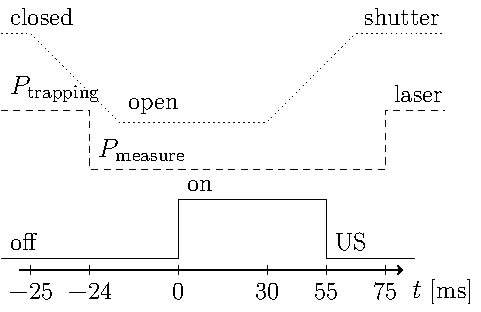
\includegraphics[]{/daq-sync.pdf}
  \caption{Schematic of controller timings for the shutter, the laser, and the 
      US. During the $P_{\text{measure}}$ state the particle is not trapped by 
  the OT. In the time interval $[\SI{0}{\ms}, \SI{30}{\ms}]$ (1) the shutter is 
  fully opened, (2) the US is switched on, and (3) the particle is free to 
  move. During this interval the measurement is performed.}\label{fig:TC-daq-sync}
\end{figure}

\subsection{Controller Timing and Data Acquisition}

The data acquisition (DAQ) board NI-USB 6356 (National Instruments, Austin, TX, 
USA), the laser power, the piezo excitation voltage, and the shutter 
transmittance are actuated in a defined sequence. We use an Arduino Board with 
two 12-Bit DAC units (MCP4725, Adafruit, New York, NY, USA) for controlling the 
timing and the DC voltage for the laser. The timings are depicted in 
\cref{fig:TC-daq-sync}. For $t<-\SI{24}{\ms}$ the laser is in its high power state 
and keeps the particle fixed in position against external forces. At 
$t=\SI{-25}{\ms}$ the shutter starts opening. The opening time is specified 
with less than \SI{15}{\ms} from 0\% transmittance to 90\%. At 
$t=\SI{-24}{\ms}$ the laser power changes to its low power state. Hence, the 
particle is free to move and starts its sedimentation. At $t=\SI{0}{\ms}$ the 
US is switched on. For \SI{30}{\ms} the shutter is fully opened, the particle 
is free to move, and the US is on. Then the shutter starts to close again. In 
these \SI{30}{\ms} we measure the time evolution of the particle. At 
$t=\SI{55}{\ms}$ the US is switched off and at $t=\SI{75}{\ms}$ the laser power 
is increased to its high power state. The time between two consecutive 
measurements is greater than \SI{2}{\s}, such that the fluid within the cavity 
is fully at rest again.

\subsection{Device, Particles, and Fluid}

Our device is a glass-silicon-glass device manufactured by Gesim GmbH 
(Radeberg, Germany). The material of the two glasses is B33 from Schott (Mainz, 
Germany). A sketch is shown in \cref{fig:TC-device} and its dimensions are listed 
in \cref{tab:TC-device-dimensions}. The top glass and the fluid cavity are limited 
in the $\ez$ direction because our microscope setup cannot focus deeper than 
\SI{250}{\um} \cite{Lamprecht2016,Lamprecht2017}. We define the origin of our 
coordinate system so that $z = 0$ is in the middle of the fluid cavity and $y = 
0$ is in the middle between the silicon cavity walls. We use as a reference 
point $x = 0$ such that it is approximately in the middle of the PZT length 
$l$. For all reported measurements we use the same position $x_{\text{ref}}$ as 
reference for $x=0$.

The fluid cavity is in the middle between the two silicon layers and the 
PZT is a PZ 26 element from Meggit A/S (Kvistgaard, 
Denmark). It is glued with Epo-Tek (Billerica, MA, USA) H20S two component 
epoxy onto the device. It is located at the edge of the device in $\ey$ 
direction and centered along the long side. The small height of 
the PZT is necessary to prevent physical contact with the microscope lens.

Our particles are silicon-dioxide (\SiO) particles from (microParticles GmbH, 
Berlin, Germany) with a diameter of $D_{2}=\SI{2.06}{\um}$. For the device 
characterization we also use particles from the same manufacturer with the same 
material properties, but with a diameter of $D_{4} = \SI{4.39}{\um}$. The 
particles are immersed in filtered (\SI{0.2}{\um}) and distilled water. To 
avoid particle-particle interactions during the experiment, we keep the 
particle concentration low.

We use the \Dtwo~particles because they are the smallest particles that work 
well in our OT. In addition, the critical radius where the ARF equals the drag 
force from AS can be found via \cite{Barnkob2012}
\begin{equation}
  \R_{\text{crit}} = \sqrt{\frac{3}{\Phi}}\,\delta
\end{equation}
where $\Phi$ is the acoustic contrast factor with thermoviscous correction 
\cite{Settnes2012}




\begin{subequations}
\begin{eqnarray}
  \Phi\left( \tkappa, \trho, \tdelta \right) &=& \frac{1}{3} f_{1}\left( 
  \tkappa \right) + \frac{1}{2}\,\text{Re}\left[ f_{2}\left( \trho, 
  \tdelta\right) \right],\\
  %%%%%%
  f_{1}\left( \tkappa \right) &=& 1 - \tkappa, \quad 
  \tkappa=\frac{\kappa_{\text{p}}}{\kappa_{\text{f}}},\\
  %%%%%%
  f_{2}\left( \trho, \tdelta \right) &=& \frac{2\left[ 1-\Gamma\left( \tdelta 
  \right) \right]\left( \trho-1 \right)}{2\,\trho + 1 - 3\,\Gamma\left( \tdelta 
  \right)}, \quad \trho=\frac{\rhop}{\rhof}\\
  %%%%%%
  \Gamma\left( \tdelta \right) &=& -\frac{3}{2}\left[ 1 + \iu \left( 1 + 
  \tdelta \right) \right]\tdelta, \, \tdelta = \frac{\delta}{R}, \, \delta = 
  \sqrt{\frac{\muef}{\rhof\,\pi f}}.
%
\end{eqnarray}
\end{subequations}
Here $\kappa_{\text{p}}$ is the particle and $\kappa_{\text{f}}$ the fluid 
compressibility, $\delta$ the VBL thickness, and $\iu$ the 
imaginary unit. For our parameters (see \cref{tab:TC-parameters}) 
$\R_{\text{crit}} $ is equal to \SI{0.63}{\um} and \SI{0.65}{\um}, with and 
without ($\tdelta = 0$) thermoviscous correction, respectively.

With increasing particle size, two effects take place: 1) the ratio between ARF 
($\propto \R^{3}$) and AS ($\FAS\propto \R$) magnitude increases, because of 
their respective scaling, and 2) the measurement time decreases, because a 
greater ARF leads to more displacement, which in turn makes re-trapping more 
difficult.

% \begin{equation}
%   \delta = \sqrt{\frac{\muef}{\pi\,\rhof\,\fex}}
% \end{equation}

% \begin{equation}
%   \Phi = \frac{1}{3}\left[ \frac{5\,\tilde{\rho}-2}{2\,\tilde{\rho}+1} - 
%   \tilde{\kappa} \right]
% \end{equation}



\afterpage{

\begin{figure}[H]
  \centering
  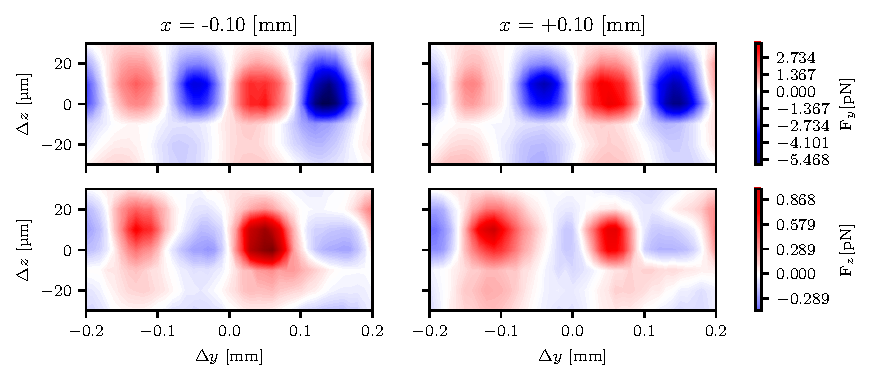
\includegraphics[width=\figWidthDouble]{\relPath/10_Figures/4um.pdf}
  % \input{10_Figures/PGF/4um_map.pgf}
  \caption{Measured steady-state acoustic forces for a \Dfour~particle with 
    $\fex=\SI{4.015}{\MHz}$ and $V_{\text{pp}} = \SI{10.7}{\volt}$. The top row 
    depicts the forces along $\ey$ and the bottom along $\ez$. The two columns 
    correspond to two different measurement $yz$-planes at $x=\SI{-0.1}{\mm}$ 
  and $x=\SI{0.1}{\mm}$, respectively.}\label{fig:4um-map}
\end{figure}

\begin{figure}[H]
  \centering
  % \input{10_Figures/PGF/2um_map.pgf}
  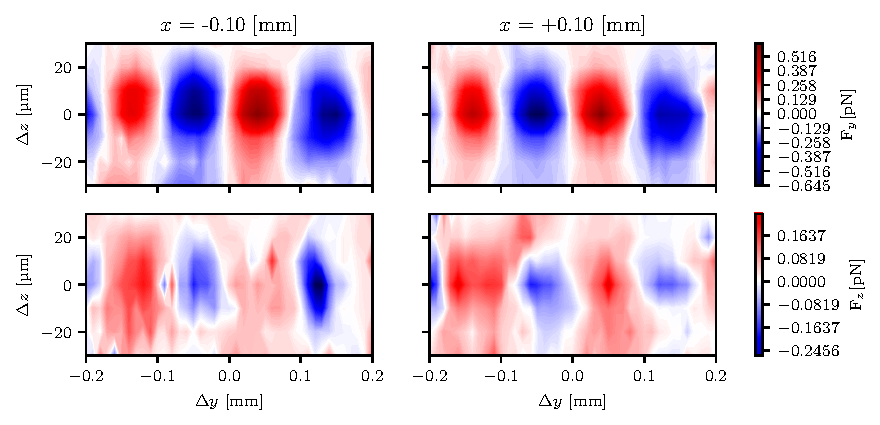
\includegraphics[width=\figWidthDouble]{\relPath/10_Figures/2um.pdf}
  \caption{Measured steady-state acoustic forces for a \Dtwo~particle with 
    $\fex=\SI{4.015}{\MHz}$ and $V_{\text{pp}} = \SI{10.7}{\volt}$. The top row 
    depicts the forces along $\ey$ and the bottom along $\ez$. The two columns 
  correspond to two different measurement $yz$-planes at $x=\SI{-0.1}{\mm}$ and 
$x=\SI{0.1}{\mm}$, respectively.}\label{fig:2um-map}
\end{figure}
\clearpage
}

\subsection{Stationary Force Measurement}
In preparation for the time evolution measurement, where a spatial position of 
orthogonal AS forces and ARFs is beneficial, we characterized our device with 
two sets of stationary force measurements at a constant excitation frequency. 
For those measurements the optical trapping force is greater than the acoustic 
forces. One measurement was with a \Dtwo, and the other with a \Dfour~diameter 
particle. For changing the particle size we needed to empty and refill the 
device.  We kept the ambient conditions and experiment settings between the two 
measurements as constant as possible. For the measurements with the 
\Dtwo~particle the ambient temperature was \SI{24.49}{\celsius} in average with 
a standard deviation of \SI{0.10}{\celsius} and for the measurement with the 
\Dfour~particle the average temperature was \SI{24.78}{\celsius} with a 
standard deviation of \SI{0.25}{\celsius} ensuring the same experimental 
conditions for both measurements. More details regarding the protocol of those 
measurements can be found in \cite{Lamprecht2016} by 
\citeauthor{Lamprecht2016}.

We defined two $yz$ measurement planes, with $x_{1} = \SI{-0.1}{\mm}$ and 
$x_{2} = \SI{0.1}{\mm}$, respectively. In each plane we defined a grid in 
$y_{i} \in \{-0.20,0.19,\dots,0.20\}\, \si{\mm}$ and $z_{j} \in 
\{-30,-20,\dots,30\}\,\si{\um}$. At each point $(y_{i}, z_{j})$ we measured the 
forces in all three dimensions 5 times for \SI{3}{\second} each. Our excitation 
frequency was set to $\fex = \SI{4.015}{\MHz}$ and the applied voltage was 
$U_{\text{pp}} = \SI{10.7}{\volt}$. We choose $\fex$ based on a frequency sweep 
and the corresponding maximal forces in this sweep. With the chosen $\fex$ and 
the fluid speed of sound $\cfl \approx \SI{1500}{\meter\per\second}$, we obtain 
the theoretical acoustic wavelength of $\lap = \sfrac{\cfl}{\fex} \approx 
\SI{375}{\um}$. Hence, with the frequency $\fex$ and a channel width of $W = 
\SI{3}{\mm}$, 16 pressure nodal lines are present. For each spatial position we 
averaged the forces over the \SI{3}{\second} timespan and also over the 5 
repetitions.

\Cref{fig:4um-map,fig:2um-map} visualize stationary force measurement results 
as contour plots for the two particle sizes. In addition, 
\Cref{fig:averaged_forces_vs_dy} depicts the measured forces in $\ey$ and $\ez$ 
directions, when the data is additionally averaged over the 7 different heights 
$\Dz$. For \Cref{subfig:F_y,subfig:F_z}, the left vertical axis is the scale 
for the \Dfour~particle and the right vertical axis for \Dtwo~particles.

In \Cref{subfig:F_y} the force wavelength $\laF$ is estimated to be 
\SI{180}{\um} which is in line with the theoretical wavelength $\laF = 
\sfrac{\lap}{2}$. One can also note that the shape of two force measurements is 
consistent. The ratio of the mean maximal force amplitudes $\frac{1.25}{0.17} = 
7.13$ is about the same as the ratio of the cubed diameter
\begin{equation}
  {\left( \frac{\Dfour}{\Dtwo} \right)}^{3} \approx 2.13^{3} \approx 9.68
 \label{eq:TC-ARF-AS-scaling}
\end{equation}
Based on the theoretical scaling laws we conclude that the forces in the $\ey$ 
direction are ARF dominant.


In \Cref{subfig:F_z} one can see the measured forces in $\ez$ for both particle 
sizes and both measurement $yz$ planes. As for the forces in $\ey$ direction, 
in \Cref{subfig:F_y}, the forces in $\ez$ direction are averaged over all 
$\Dz$. The force magnitude for both sizes is smaller than in $\ey$ direction 
for both particle sizes. The shapes, however, are similar but not as consistent 
as in \Cref{subfig:F_y}. The ratio of the mean maximal force amplitudes 
$\frac{0.25}{0.08} \approx 3.1$ is about the same as the ratio of the two 
diameters, which suggests that in the $\ez$ direction the forces on the 
particle are AS dominated (see \Cref{eq:TC-ARF-AS-scaling}).

\begin{figure}[H]
  \centering
  \begin{subfigure}{\figWidth}
    \centering
    \caption{$F_{y}$ [\si{\pico\newton}]}\label{subfig:F_y}
    % \tikzsetnextfilename{avgF_y_vs_dy}
\begin{tikzpicture}
  \begin{axis}[%
      scale only axis,
      width = 60mm,
      height = 5cm,
      axis y line*=left,
      legend style={
        fill=blue!10!white,
        font=\tiny,
        at={(0.03,0.05)},
        anchor=south west},
      xlabel = {$\Dy$ [\si{\mm}]}]

    \fill[fill=black!15!white] ({axis cs:-0.06,-2}|-{rel axis cs:0,0}) 
    rectangle ({axis cs:-0.03,2}|-{rel axis cs:0,1});

    \addlegendimage{empty legend}
    \addlegendentry{\hspace{-.6cm}\textbf{$\Rfour$}}

    \addplot[thick, blue] table[x=dy, y=F4_y1] 
    {\relPath/10_Figures/TikZ/averaged_yz_Forces.dat};
    \addlegendentry{$x_{1}$};

    \addplot[thick, blue, dashed] table[x=dy, y=F4_y2] 
    {\relPath/10_Figures/TikZ/averaged_yz_Forces.dat};
    \addlegendentry{$x_{2}$};


    \draw[|<->|] ({axis cs:-0.135,0}|-{rel axis cs:0,0.95}) -- ({axis 
    cs:0.05,0}|-{rel axis cs:0,0.95}) node[midway,below] 
    {$\sfrac{\lap}{2}=\laF$};


  \end{axis}
  \pgfplotsset{every axis y label/.append style={rotate=180,yshift=86mm}}
  \begin{axis}[%
      scale only axis,
      width = 60mm,
      height = 5cm,
      legend style={
        fill=lightgray,
        font=\tiny,
        at={(0.97,0.95)},
        anchor=north east},
      axis x line=none,
    axis y line*=right]

    \addlegendimage{empty legend}
    \addlegendentry{\hspace{-.6cm}\textbf{$\Rtwo$}}

    \addplot[thick, dotted] table[x=dy, y=F2_y1] 
    {\relPath/10_Figures/TikZ/averaged_yz_Forces.dat};
    \addlegendentry{$x_{1}$};

    \addplot[thick,loosely dashed] table[x=dy, y=F2_y2] 
    {\relPath/10_Figures/TikZ/averaged_yz_Forces.dat};
    \addlegendentry{$x_{2}$};

  \end{axis}
\end{tikzpicture}

    % \includegraphics[width=\subfigWidth]{Plots/cache/avgF_y_vs_dy.eps}
    \includegraphics[]{Plots/cache/avgF_y_vs_dy.eps}
  \end{subfigure}%
  \begin{subfigure}{\figWidth}
    \centering
    % \tikzsetnextfilename{avgF_z_vs_dy}
\begin{tikzpicture}
  \begin{axis}[%
      scale only axis,
      width = 60mm,
      height = 5cm,
      axis y line*=left,
      legend style={
        fill=blue!10!white,
        font=\tiny,
        at={(0.03,0.05)},
        anchor=south west},
      xlabel = {$\Dy$ [\si{\mm}]}]

    \fill[fill=black!15!white] ({axis cs:-0.06,-2}|-{rel axis cs:0,0}) 
    rectangle ({axis cs:-0.03,2}|-{rel axis cs:0,1});

    \addlegendimage{empty legend}
    \addlegendentry{\hspace{-.6cm}\textbf{$\Rfour$}}

    \addplot[thick,blue] table[x=dy, y=F4_z1] 
    {\relPath/10_Figures/TikZ/averaged_yz_Forces.dat};
    \addlegendentry{$x_{1}$};

    \addplot[thick, blue, dashed] table[x=dy, y=F4_z2] 
    {\relPath/10_Figures/TikZ/averaged_yz_Forces.dat};
    \addlegendentry{$x_{2}$};

  \end{axis}
  \pgfplotsset{every axis y label/.append style={rotate=180,yshift=86mm}}
  \begin{axis}[%
      scale only axis,
      width = 60mm,
      height = 5cm,
    axis y line*=right,
      yticklabel style={
        /pgf/number format/fixed,
        /pgf/number format/precision=2
      },
      legend style={
        fill=lightgray,
        font=\tiny,
        at={(0.97,0.95)},
        anchor=north east},
      axis x line=none]

    \addlegendimage{empty legend}
    \addlegendentry{\hspace{-.6cm}\textbf{$\Rtwo$}}

    \addplot[thick, dotted] table[x=dy, y=F2_z1] 
    {\relPath/10_Figures/TikZ/averaged_yz_Forces.dat};
    \addlegendentry{$x_{1}$};

    \addplot[thick,loosely dashed] table[x=dy, y=F2_z2] 
    {\relPath/10_Figures/TikZ/averaged_yz_Forces.dat};
    \addlegendentry{$x_{2}$};

  \end{axis}
\end{tikzpicture}

    % \includegraphics[width=\subfigWidth]{Plots/cache/avgF_z_vs_dy.eps}
    \caption{$F_{z}$ [\si{\pico\newton}]}\label{subfig:F_z}
    \includegraphics[]{Plots/cache/avgF_z_vs_dy.eps}
  \end{subfigure}%
  \caption{Measured steady-state acoustic forces when averaged over the cavity 
    height. All values are in \si{\pico\newton}. For each plot the left 
    $y$-axis is the measured force on the \Dfour~($D_{4}$) particle and the 
    right one for the \Dtwo~($D_{2}$) particle, respectively.
    The gray shaded area corresponds to the positions where the time evolution 
  is measured.}\label{fig:averaged_forces_vs_dy}
\end{figure}

\subsection{Measurement Protocol for Time Evolution}

Based on a set of proof-of-concept experiments (data not shown here) and the 
information from numerical simulations that the AS field in a \emph{real} 
device can substantially differ from the AS field of fluid cavity-only 
structure, we selected $x = 0$, $y_{i} \in 
\{-0.15,-0.14,\dots,0.10\}\,\si{\mm}$, and $z_{j} \in \{-10,0,10\}\,\si{\um}$. 
This choice means, that we measure at the same $y_{i}$ and $z_{j}$ as for the 
stationary force measurement. We have the same excitation frequency ($\fex = 
\SI{4.015}{\MHz}$) as in the stationary force measurements from before. However 
we set the excitation amplitude slightly higher to $U_{\text{pp}} = 
\SI{11.7}{\volt}$ in order to increase the signal to noise ratio (SNR).

We control the whole measuring routine with a self-written Python program. 
Before each measurement, the offset of the QPDs is checked and, if needed, 
adjusted. First we measure without US and then we measure with US on. We repeat 
this procedure 50 times before moving to the next location.

For the time evolution measurement, we acquire with a sampling rate of $\fs 
=\SI{1.25}{\MHz}$ ($\Dt = \SI{0.8}{\us}$) for \SI{125}{\ms} the three QPD 
signals, the signal for the shutter, and the DC signal for the laser as soon as 
the shutter starts opening ($t = \SI{-25}{\ms}$ in \Cref{fig:daq-sync}). 
Between $t =\SI{0}{\ms}$ and $t = \SI{30}{\ms}$ the shutter is completely open 
and the US is switched on. Extending the measurement time further has no 
benefit because the particle will be outside the linear regimes of the QPDs and 
might move too far from the OT trapping region such that it cannot be 
recaptured after the laser changes to its high power state again.

We repeat 50 times per position because the particle starts sedimenting 
as soon as the laser power drops to the lower value. During this movement the 
particle still undergoes Brownian motion. Hence, the trajectory is not straight 
along the $\ez$ direction. With 50 datasets, we can average this random 
movement out.

Taking the approximation of \cref{eq:TC-mod-free-fall} into account, a \Dtwo~large 
\SiO~sphere sedimenting in water reaches its terminal velocity 
almost instantaneously, because the inertia term is small; additionally, the 
sphere travels about $0.12\,\Rtwo$ in \SI{55}{\ms}. Therefore, after 
\SI{25}{\ms} the particle is still in the linear regime of the QPDz. The static 
gravitational force ($\tilde{m}g$) with the added buoyancy of water is less 
than \SI{40}{\femto\newton} for the \Dtwo~particle. This is more than 6 times 
smaller than the maximal measured force in $\ez$ direction. Therefore, we 
assume in areas of maximal forces along $\ez$ that the driving force of this 
movement is either the acoustic field or $\FAS$. With an ideal sedimentation in 
the first \SI{25}{\ms} along $\ez$, the laser spot on QPDxy does not change at 
all during the sedimentation.

\subsection{Data Processing}

The acquired data is postprocessed with Python. We look at discrete points 
every $t_{k} = k\cdot\SI{0.1}{\ms}$ with $k\in \mathbb{N}$. In addition, we use 
a moving average for the data at $t_{k}$ with a centered window size of 101 
data points, corresponding to a timespan of \SI{80}{\us}. Next, we subtract the 
data series without US from the series with US to obtain the delta voltage 
$\DV_{m}$, with $m$ being $y$ or $z$. This quantity allows us to further reduce 
unwanted noise. This step serves also as data quality check because all 
measurements have the same protocol until $t=\SI{0}{\ms}$. Hence, the delta 
voltage $\DV_{m}$ must be \emph{zero} for $t\leq\SI{0}{\ms}$. Then, we average 
$\DV_{m}$ over the 50 repetitions per spatial position $y_{i}, z_{j}$. As last 
step for the time evolution plots, we normalize the data by the $\max\left( 
\left\vert \DV_{m}(t)\right\vert \right)$ for $\SI{10}{\ms} < t < 
\SI{30}{\ms}$.

\section{Results and Discussion\label{sec:TC-results}}

\Cref{subfig:res_DV_y} shows that the maximal averaged voltage difference 
$\DV_{y}$ for the \Dtwo~particle while having the leaser in the 
$P_{\text{measure}}$ mode. It has the same shape as the stationary force 
measurement in \cref{subfig:F_y}.  However, the smoothness of $\DV_{y}$ is 
worse. We attribute this to the nature of the experiment, as the recorded 
motion of the particle is caused by two effects; one is the acoustic field and 
the other is the always present Brownian motion.  For the stationary force 
measurements the particle is fixed in place by the optical potential and the 
Brownian motion is negligible.

By measuring the same shape with the two experiments, we could validate our 
measurement protocol. As for the stationary measurements, the SNR of the 
evolution measurement and also shape are better for the in-plane $\ey$ than the 
axial $\ez$ (see \cref{subfig:F_y} and \cref{subfig:F_z}). Nevertheless, 
\cref{subfig:F_z} and \cref{subfig:res_DV_z} also show similar shapes. We want 
to stress again, that the amplitudes of \cref{fig:DV_vs_dy} are not comparable 
to each other for $\ey$ and $\ez$ (see \cref{sec:TC-experimental-setup}).
% This step enables data comparability, because the raw magnitudes are 
% inherently different. As stated before, the in-plane position detection along 
% $\ex$ and $\ey$ functions differently than the axial along $\ez$.

The numerical streaming simulations of a fluid cavity with and without the
surrounding structure showed that the streaming field is a local effect in a
model with surrounding structure. In our experiments we saw similar tendencies.  
However, not all measured spatial locations had enough actual signal strength 
to further investigate. In \Cref{fig:evolutioin-V} we plot the time evolution 
of the signal for four different $\Dy$ where it is clear that the signal is due 
to the acoustic field and not to noise or Brownian motion.

\begin{figure}[ht]
  \centering
  \begin{subfigure}{\figWidth}
    \centering
    \caption{Data for $y$-component ($m = y$)}\label{subfig:res_DV_y}
    % \tikzsetnextfilename{avgV_y_vs_dy}
\begin{tikzpicture}
  \begin{axis}[%
      scale only axis,
      width = 60mm,
      height = 45mm,
      xticklabel style={
        /pgf/number format/fixed,
        /pgf/number format/precision=2
      },
      legend style={
        fill=lightgray,
        font=\tiny,
        at={(0.97,0.05)},
        anchor=south east
      },
      legend cell align={left},
      ylabel={$\max\left( \DV_{m}\left( t \right) \right)$ [\si{\mV}]},
      xlabel = {$\Dy$ [\si{\mm}]}]

      \fill[fill=black!15!white] ({axis cs:-0.065,-0.0002}|-{rel axis cs:0,0}) 
      rectangle ({axis cs:-0.025,0.0002}|-{rel axis cs:0,1});

    \addplot[thick,mark=*,mark size=1pt] table[x=dy, y=DV_y_m10] 
    {\relPath/10_Figures/TikZ/averaged_yz_mVoltages.dat};
    \addlegendentry{$\Dz = -10$};

    \addplot[thick, dotted,mark=*,mark size=1pt] table[x=dy, y=DV_y_m00] 
    {\relPath/10_Figures/TikZ/averaged_yz_mVoltages.dat};
    \addlegendentry{$\Dz = 0$};

    \addplot[thick, dashed,mark=*,mark size=1pt] table[x=dy, y=DV_y_p10] 
    {\relPath/10_Figures/TikZ/averaged_yz_mVoltages.dat};
    \addlegendentry{$\Dz = +10$};

    % wavelength
    \draw[|<->|] ({axis cs:-0.135,0}|-{rel axis cs:0,0.55}) -- ({axis 
    cs:0.05,0}|-{rel axis cs:0,0.55}) node[midway,above] 
    {$\sfrac{\lap}{2}=\laF$};

  \end{axis}
\end{tikzpicture}

    \includegraphics[]{Plots/cache/avgV_y_vs_dy.eps}
  \end{subfigure}%
  \begin{subfigure}{\figWidth}
    \centering
    \caption{Data for $z$-component ($m = z$)}\label{subfig:res_DV_z}
    % \tikzsetnextfilename{avgV_z_vs_dy}
\begin{tikzpicture}
  \begin{axis}[%
      scale only axis,
      width = 60mm,
      height = 45mm,
      xticklabel style={
        /pgf/number format/fixed,
        /pgf/number format/precision=2
      },
      legend style={
        fill=lightgray,
        font=\tiny,
        at={(0.97,0.05)},
        anchor=south east
      },
      legend cell align={left},
      xlabel = {$\Dy$ [\si{\mm}]}]

      \fill[fill=black!15!white] ({axis cs:-0.065,-0.0002}|-{rel axis cs:0,0}) 
      rectangle ({axis cs:-0.025,0.0002}|-{rel axis cs:0,1});

    \addplot[thick,mark=*,mark size=1pt] table[x=dy, y=DV_z_m10] 
    {\relPath/10_Figures/TikZ/averaged_yz_mVoltages.dat};
    \addlegendentry{$\Dz = -10$};

    \addplot[thick, dotted,mark=*,mark size=1pt] table[x=dy, y=DV_z_m00] 
    {\relPath/10_Figures/TikZ/averaged_yz_mVoltages.dat};
    \addlegendentry{$\Dz = 0$};

    \addplot[thick, dashed,mark=*,mark size=1pt] table[x=dy, y=DV_z_p10] 
    {\relPath/10_Figures/TikZ/averaged_yz_mVoltages.dat};
    \addlegendentry{$\Dz = +10$};

  \end{axis}
\end{tikzpicture}

    \includegraphics[]{Plots/cache/avgV_z_vs_dy.eps}
  \end{subfigure}%
  \caption{Maximal $\DV_{y}$ and $\DV_{z}$ averaged over all repetitions in the 
    timespan between \SI{35}{\ms} and \SI{55}{\ms} for the three different 
    measurement heights $\Dz = \SIlist[list-units=single, list-final-separator 
    = {, }, list-pair-separator= {, }] {-10;0;10}{\um}$. The gray shaded area 
    represents the $\Dy_{i}$ of best signal strength for $\max\left( 
    \DV_{z}\left( t \right) \right)$. The data points of best strength are 
    taken for the time evolution results. The wavelength marker represents the 
  same length as in \cref{subfig:F_y}.}\label{fig:DV_vs_dy}
\end{figure}%

Since we show $\DV_{m}$ rather than the absolute voltage amplitudes, we can 
further validate our protocol. For $\sfrac{t}{t_{0}} < 0$, where $t_{0} = 
\sfrac{1}{\fex}$ and $\sfrac{t}{t_{0}}=0$ represents the time when the US is 
switched on (in \cref{fig:daq-sync} $t = \SI{0}{\ms}$), all data series in 
\cref{fig:evolutioin-V} are zero. All data series for $\ez$ are more noisy than 
for $\ey$. However, we also have the same amplitude of noise in $\ey$ 
direction. But, the normalization value for the data series for $\ey$ is 
inherently larger than for $\ez$ (see \cref{fig:DV_vs_dy}).

\afterpage{
\begin{figure}[ht]
  \centering
  % \tikzsetnextfilename{evolution_V}
%%%%%%%
% READ TABLE
%%%%%%%
\pgfplotstableread{\relPath/10_Figures/TikZ/evolution_yz_Voltages.dat}{\data}
%%%%%%%
% LINES FOR ALL GROUPPLOTS
%%%%%%%
\renewcommand{\tikzHelper}{
  \fill[fill=black!10!white] (axis cs:-80,0) rectangle (axis cs:0,1);

  \draw[dotted] (axis cs:0,0) -- (axis cs:0,1);
  \draw[dotted] (axis cs:50,0) -- (axis cs:50,1);
  \draw[dotted] (axis cs:100,0) -- (axis cs:100,1);
  \draw[dotted] (axis cs:-80,0.5) -- (axis cs:120,0.5);
  \draw[dotted] (axis cs:-80,0.5) -- (axis cs:120,0.5);
}



\begin{tikzpicture}
   \begin{groupplot}[%
       scale only axis,
       group style={
         group size= 2 by 4,
         group name=plots,
         vertical sep=4pt,%
         horizontal sep=8pt},%
       height=40mm,%
       width=64mm,%
        xticklabel style={
          /pgf/number format/fixed,
          /pgf/number format/precision=2
        }]

%%%%%%
%%% PLOT (1,1)
%%%%%%

   \nextgroupplot[%
      legend style={
        fill=lightgray,
        font=\tiny,
        at={(0.03,0.95)},
        anchor=north west
      },
      legend cell align={left},
     xticklabels={,,},
     % title={$\DV_{y}\,|\,\Dy = \SI{-0.06}{\milli\meter}$},%
     title={Data for $y$-component ($m = y$)},%
     ylabel={$\sfrac{\DV_{m}}{\DV_{m,\text{max}}}$}]

      \tikzHelper
      \draw[thick,|<->|] (axis cs:-80,0.25) -- (axis cs:0,0.25) node[midway, 
      above] {US off};

      \addplot[thick] table[x=dt, y=DV_y_m06_m10] {\data};

      \addplot[thick, dotted] table[x=dt, y=DV_y_m06_m00] {\data};

      \addplot[thick, dashed] table[x=dt, y=DV_y_m06_p10] {\data};

      \addlegendentry{$\Dz = \SI{-10}{\um}$};
      \addlegendentry{$\Dz = \SI{0}{\um}$};
      \addlegendentry{$\Dz = \SI{+10}{\um}$};



%%%%%%
%%% PLOT (1,2)
%%%%%%

   \nextgroupplot[%
     xticklabels={,,},
     yticklabels={,,},
     title={Data for $z$-component ($m = z$)}]%
   % title={$\DV_{z}\,|\,\Dy = \SI{-0.06}{\milli\meter}$}]

      \tikzHelper

      \addplot[thick] table[x=dt, y=DV_z_m06_m10] {\data};

      \addplot[thick, dotted] table[x=dt, y=DV_z_m06_m00] {\data};

      \addplot[thick, dashed] table[x=dt, y=DV_z_m06_p10] {\data};

%%%%%%
%%% PLOT (2,1)
%%%%%%

   \nextgroupplot[%
     xticklabels={,,},
     ylabel={$\sfrac{\DV_{m}}{\DV_{m,\text{max}}}$ },
     % title={$\Dy = \SI{-0.05}{\milli\meter}$}
   ]

      \tikzHelper

      \addplot[thick] table[x=dt, y=DV_y_m05_m10] {\data};

      \addplot[thick, dotted] table[x=dt, y=DV_y_m05_m00] {\data};

      \addplot[thick, dashed] table[x=dt, y=DV_y_m05_p10] {\data};

%%%%%%
%%% PLOT (2,2)
%%%%%%

   \nextgroupplot[%
     xticklabels={,,},
     yticklabels={,,},
     % title={$\Dy = \SI{-0.05}{\milli\meter}$}
   ]

      \tikzHelper

      \addplot[thick] table[x=dt, y=DV_z_m05_m10] {\data};

      \addplot[thick, dotted] table[x=dt, y=DV_z_m05_m00] {\data};

      \addplot[thick, dashed] table[x=dt, y=DV_z_m05_p10] {\data};

%%%%%%
%%% PLOT (3,1)
%%%%%%

   \nextgroupplot[%
     xticklabels={,,},
     ylabel={$\sfrac{\DV_{m}}{\DV_{m,\text{max}}}$ },
     % title={$\Dy = \SI{-0.04}{\milli\meter}$}
   ]

      \tikzHelper

      \addplot[thick] table[x=dt, y=DV_y_m04_m10] {\data};

      \addplot[thick, dotted] table[x=dt, y=DV_y_m04_m00] {\data};

      \addplot[thick, dashed] table[x=dt, y=DV_y_m04_p10] {\data};

%%%%%%
%%% PLOT (3,2)
%%%%%%

   \nextgroupplot[%
     xticklabels={,,},
     yticklabels={,,},
     % title={$\Dy = \SI{-0.04}{\milli\meter}$}
   ]

      \tikzHelper

      \addplot[thick] table[x=dt, y=DV_z_m04_m10] {\data};

      \addplot[thick, dotted] table[x=dt, y=DV_z_m04_m00] {\data};

      \addplot[thick, dashed] table[x=dt, y=DV_z_m04_p10] {\data};


%%%%%%
%%% PLOT (4,1)
%%%%%%

   \nextgroupplot[%
     ylabel={$\sfrac{\DV_{m}}{\DV_{m,\text{max}}}$},
     xlabel={$10^{3}\,\sfrac{t}{t_{0}}$ },
     % title={$\Dy = \SI{-0.03}{\milli\meter}$}
   ]

      \tikzHelper

      \addplot[thick] table[x=dt, y=DV_y_m03_m10] {\data};

      \addplot[thick, dotted] table[x=dt, y=DV_y_m03_m00] {\data};

      \addplot[thick, dashed] table[x=dt, y=DV_y_m03_p10] {\data};

%%%%%%
%%% PLOT (4,2)
%%%%%%

   \nextgroupplot[%
     yticklabels={,,},
     xlabel={$10^{3}\,\sfrac{t}{t_{0}}$},
     % title={$\Dy = \SI{-0.03}{\milli\meter}$}
   ]

      \tikzHelper

      \addplot[thick] table[x=dt, y=DV_z_m03_m10] {\data};

      \addplot[thick, dotted] table[x=dt, y=DV_z_m03_m00] {\data};

  \end{groupplot}

%%%%%%
%%% TEXT NEXT TO PLOTS
%%%%%%
  \node[rotate=90] at (plots c2r1.east) [yshift=-5mm] {$\Dy = 
  \SI{-0.06}{\milli\meter}$};
  \node[rotate=90] at (plots c2r2.east) [yshift=-5mm] {$\Dy = 
  \SI{-0.05}{\milli\meter}$};
  \node[rotate=90] at (plots c2r3.east) [yshift=-5mm] {$\Dy = 
  \SI{-0.04}{\milli\meter}$};
  \node[rotate=90] at (plots c2r4.east) [yshift=-5mm] {$\Dy = 
  \SI{-0.03}{\milli\meter}$};

\end{tikzpicture}

  \includegraphics[]{Plots/cache/evolution_V.eps}
  \caption{Time evolution of the normalized $\DV_{y}$ (left column) and 
    $\DV_{z}$ (right column) for the three measurement heights $\Dz = 
    \SIlist[list-units=single, list-final-separator = {, }, 
    list-pair-separator= {, }] {-10;0;10}{\um}$ and the positions for $\Dy = 
    \SIlist[list-units=single, list-final-separator = {, }, 
    list-pair-separator= {, }] {-0.06;-0.05;-0.04;-0.03}{\mm}$. The gray shaded 
    area of each plot marks the time when the US is off; 
  $t_{0}=\sfrac{1}{\fex}$.}\label{fig:evolutioin-V}
\end{figure}
}

For all 12 positions $(y_{i}, z_{j})$ in \cref{fig:evolutioin-V} the signal 
along $\ey$ starts changing as soon as the US is switched on. This 
is in line with the estimation of \cref{eq:TC-tau-arf} for $\tarf$. For all data 
series $m = z$ it takes significantly more time until the movement with 
constant velocity starts. To further compare the results, we take as criteria 
the period $p^{\ast} = \sfrac{t^{\ast}}{t_{0}}$, when the normalized $\DV_{m} 
\ge 0.5$ is reached. In \cref{tab:TC-results}, the absolute periods for this 
criteria and the offset between the movement along $\ey$ ($m=z$) and the 
movement along $\ez$ ($m=y$) are shown. Taking a different criteria value 
(e.g., the normalized $\DV_{m} \ge 0.3$) changes the absolute magnitude of the 
values $p^{\ast}$, however the offset does not change significantly. The 
average for all $\Delta p^{\ast}$ is about 17'500 which equates to $\approx 
\SI{4.35}{\ms}$ for the excitation frequency $\fex = \SI{4.015}{\MHz}$.

\begin{table*}
  \centering
  \begin{tabular}{ll *{4}{x{27mm}}}
    \toprule
    \toprule
  {\bfseries $\Dy$} & [\si{\mm}] & -0.06 & -0.05 & -0.04 & -0.03 \\

    \midrule
    % {\small
  {\bfseries $p^{\ast}_{y}$ } & ($\times 1000$) [-] & 64.2, 69.5, 70.7 & 65.8, 
  70.3, 70.3 & 65.8, 60.6, 76.7 & 73.5, 57.4, 74.3 \\[2mm]

  {\bfseries $p^{\ast}_{z}$} & ($\times 1000$) [-] & 80.7, 87.9 88.3 & 86.3, 
  85.5, 86.7 & 83.1, 89.5, 87.5 & 87.9, 86.7,  \\

    \midrule
    
  {\bfseries $\Delta p^{\ast}$} & ($\times 1000$) [-] & 16.5, 18.4, 17.6 & 
  20.5, 15.2, 16.4 & 17.3, 18.9, 10.8 & 14.4, 29.3, \\
    % }
    \bottomrule
    \bottomrule
    
  \end{tabular}
  \caption{Absolute periods $p^{\ast}_{m}$ when the normalized $\DV_{m} > 0.5$.  
    The three values per column correspond to the three heights $\Dz = 
    \SIlist[list-units=single, list-final-separator = {, }, 
    list-pair-separator= {, }] {-10;0;10}{\um}$ per $\Dy$ respectively. For 
  $\Dy = \SI{-0.03}{\mm}$ and $\Dz = \SI{10}{\um}$ no data is available for 
$p_{z}^{\ast}$. The last row states the offset $\Delta p^{\ast} = p^{\ast}_{z} 
- p^{\ast}_{y}$}\label{tab:TC-results}
\end{table*}

In addition, all slopes for the $y$ movement ($m=y$) are linear almost 
immediately after the US is
switched on. This suggests, that the ARF is constant and accelerates the 
particle fast to its terminal velocity. The measured voltages and also their 
differences are linearly related to the traveled distances. Hence, a constant 
increase in voltage, which means a constant voltage increase per time 
$\sfrac{\text{d}\,\DV_{m}}{\text{d}t} = const.$, implies a constant particle 
speed along the $\ey$ direction. The particle trajectory in $\ez$ direction is 
predominantly affected by the streaming field. This fluid motion takes more 
time until it is established. With the same reasoning as before, a linear slope 
for the $z$ movement ($m=z$) in \cref{fig:evolutioin-V} implies a constant 
force and constant particle speed. A constant speed means a non-changing 
streaming field and therefore a constant streaming velocity.


\section{Conclusion\label{sec:conclusion}}

In this work we presented the measurement of the temporal evolution of the AS 
field and the ARF in a BAW device utilizing an OT. We slightly modified our 
validated optical trapping setup \cite{Lamprecht2016,Lamprecht2021} to 
accommodate the requirements of this experiment. With a temporal resolution of 
$\Dt=\SI{0.8}{\us}$ we could measure at least every fourth time period of 
excitation. We validated our measurement protocol against the stationary force 
field.

We monitored the trajectory of a \Dtwo~\SiO~particle as soon as the US 
excitation of the device started. We selected measurement positions in a 
standing pressure wave mode where ARF dominates in one direction and AS 
orthogonal to it. In addition, we chose the spatial location within the mode 
to maximize the amplitude of both effects. Our measurements show, that the ARF 
is established almost immediately after the US is switched on; whereas the AS 
takes in average 17'500 excitation periods (\SI{4.4}{\ms}) longer to evolve. 
This time is about four times larger than the theoretical approximation with 
the momentum diffusion time.

These results show that the build up of AS takes significantly longer than the 
build up of the ARF. This temporal difference can explain why a pulsed acoustic 
excitation can prevent streaming as it has been experimentally shown by 
\citeauthor{Hoyos2013} \cite{Hoyos2013,Castro2016}. In addition, the results of 
the streaming simulations of a cavity-only model and a whole-device model show 
that simplified models are enough for simulations of the pressure fields, 
however they cannot reflect \emph{real} streaming patterns. This insight might 
also explain why \citeauthor{Muller2015} could not reproduce the suppression of 
AS with a pulsed excitation in their cavity-only model.



\cleardoublepage
\renewcommand{\relPath}{SECTION/50_Viscous_Torque}
 
\chapter[Particle Rotation Measurements with an OT]{Rotational Speed 
Measurements of Small Spherical Particles driven by Acoustic Viscous Torques 
utilizing an Optical Trap}\label{ch:viscoustorque}
\textit{For this work Andreas Lamprecht performed all measurements and sketched 
  a draft for the manuscript. Christoph Goering carried out the postprocessing 
  of the data and the whole submission and writing process.:
\footnote{: DOI: https://doi.org/10.1088/1361-6439/abde92, reproduced with 
permission, copyright 2021 IOP Publishing.}}

\vspace{5mm} \noindent
Andreas Lamprecht, Christoph Goering, Iwan A.T. Schaap, and Jürg Dual,
"Rotational speed measurements of small spherical particles driven by acoustic 
viscous torques utilizing an optical trap", Journal of Micromechanics and 
Microengineering, 2021, \textbf{34} 034004.


\section{Abstract}
Two orthogonal standing acoustic waves, generated by piezoelectric excitation, 
can form a two-dimensional pressure field in microfluidic devices. A phase 
difference of the excitation waves can be employed to rotate spherical 
\si{\micro\meter}-sized silica particles by a torque mediated through the 
viscous boundary $\delta$ around the particle.

The measurement of the rotational rate is, so far, limited to high-speed cameras 
and their frame rate, and gets increasingly difficult when the sphere gets 
smaller.  We report here a new method for measuring the rotational rate of 
\si{\micro\meter} sized spherical particles. We utilize an optical trap with 
high-speed position detection to overcome the frame rate limitation of wide 
field image recording. The power spectrum of an optically trapped, rotating 
particle reveals additional peaks corresponding to the rotational frequencies -- 
compared to a non-rotating particle. We validate our method at low rotational 
rates against high-speed video observation. 

To demonstrate the potential of this method we addressed a recent controversy 
about the rotation of particles with a relatively large VBL 
$\delta$. We measured steady-state rotational rates up to \SI{229}{\hertz} 
(\SI{13.8e3}{\rpm}) for a particle with a radius $R \approx \delta$.  Recent 
numerical research suggests that in this regime the existing theoretical 
approach (valid for $R\gg\delta$) overpredicts the steady-state rotational rate 
by a factor of 10.  With our new method we also confirm the numerical results 
experimentally.

\section{Introduction\label{sec:TC-introduction}}

In recent years, acoustofluidics has provided many powerful tools. Due to being 
contact-less, label-free, and biocompatible 
\cite{Antfolk2015,Abdulla2020,Zielke2020,Binkley2020,Cai2020}, acoustofluidic 
manipulation can be used in medical applications for cancer research
\cite{Antfolk2015,Abdulla2020,Zielke2020,Binkley2020}, Alzheimer research 
\cite{Cai2020}, targeted drug delivery \cite{Bose2015}, and for pumping medical 
fluids \cite{Wu2019}. In addition, there are biological 
\cite{Gerlt2020,Xie2019} and engineering applications (e.g., micro-pumping 
\cite{Wu2019,Huang2014,Lin2019,Ozcelik2021}).

Most of these applications utilize the acoustic radiation force (ARF) to 
manipulate objects on the micro-scale. The ARF is a second-order time-averaged 
effect that arises from the interaction of an acoustic field scattered at an 
object surface and a background acoustic field 
\cite{Doinikov1994Rigid,Hasegawa1969,Yosioka1955,Gorkov1962,Bruus2012}.
These objects can be solid particles, air bubbles, fluid droplets, biological 
samples, as long as their material properties (density $\rho$ and speed of 
sound $c$) are different from the surrounding medium. However, there coexists 
a fluid motion called acoustic streaming (AS) 
\cite{Nyborg1965,Kolb1956,Nyborg1953}. This motion can arise either from
viscous losses in the fluid (Eckhart type streaming \cite{Eckart1948}) or it 
can arise in the viscous boundary layer at a fluid to wall interface 
(Schlichting and Rayleigh streaming \cite{Riley1998,Schlichting1932}).


The theoretical derivations usually describe the steady-state of the AS field. 
A theoretical numerical study \cite{Muller2015} investigated the temporal build 
up of the ARF and AS field. In contrast to the ARF, the viscous drag force 
arising from AS is independent of the object material properties because it is 
a motion of the fluid. The AS direction coincides with the direction of the 
relative motion between fluid and particle.

For a spherical object of radius $R$, the drag force in laminar flow scales 
linearly with the object radius $\FAS \propto R$. In contrast to the $\FAS$, 
the ARF scales with the volume $\FARF \propto \R^{3}$ \cite{Bruus2012-10}.  
Based on the fluid and the object material properties, the $\FARF$ will 
dominate over the $\FAS$ if the radius $\R$ is greater than the critical radius 
$\R_{\text{crit}}$, where $\FAS = \FARF$ holds. The direction of $\FAS$ can be 
different from the $\FARF$. Therefore, the $\FAS$ is usually undesired.

The ARF and the AS occur not only in the bulk of the fluid, but also on sharp 
edges of a device \cite{Doinikov2020a,Doinikov2020b,Leibacher2015,Nama2016}. 
So-called micro-streaming around the surface of a spherical particle can even 
cause a sign inversion of the ARF if the viscous boundary layer $\delta$ is 
sufficiently large \cite{Baasch2019}. However, there are applications that take 
advantage of the AS \cite{Antfolk2014,Mao2017,Hao2020}: a complete overview of 
AS applications can be found in \cite{Wiklund2012a}.

In literature, it is well understood how long it takes until the acoustic 
field, and hence the ARF, needs to build up \cite{Muller2015} and how long the 
particle focusing takes \cite{Bruus2012-10}. However, it is still not fully 
clear how long it takes for the AS to build up, and what the definition for the 
analytical AS time constant is. In the acoustofluidics community, it is 
generally accepted that the build up for the AS field takes longer than the 
build up of the ARF. By using a pulsed actuation of the acoustic field and 
therefore exploiting this time offset, \citeauthor{Hoyos2013} prevented the 
build up of AS \cite{Hoyos2013,Castro2016}. They varied the number of periods 
for which the acoustic actuation is switched on and off, respectively. They 
experimentally showed that for a ratio of about 1 to 1 between 500 on- and 500 
off-periods the streaming velocity is less than 50\% of its steady-state 
magnitude while the ARF is not affected by that much.

\citeauthor{Muller2015} studied the build up of the acoustic energy density and 
streaming velocity with a numerical model \cite{Muller2015}. Their model 
consisted of a fluid cavity without any surrounding structure such as the 
cavity walls. They found numerically that indeed the ARF builds up 
significantly faster than the AS. However, the simulations with a pulsed 
actuation of different ratios of on- to off-periods did not prevent the build 
up of AS because its decay -- as the build up -- is slow compared to the ARF. 
The streaming builds up significantly slower during the on-periods, however, it 
does not decay to its initial value during the off-periods. Over time the 
influence of AS increases because the ARF alternates between some magnitude in 
the on-periods and zero in the off-periods. This implies, that the simulation 
of \citeauthor{Muller2015} could not explain the experimental results by 
\citeauthor{Hoyos2013}.

In this work, we experimentally measure the time until a \Dtwo~spherical 
silicon-dioxide (\SiO) particle moves with constant velocity when accelerated 
by the ARF and AS. Instead of using a camera, we utilize a data acquisition 
board (DAQ) with a sampling frequency of $f_{\text{s}} = \SI{1.25}{\MHz}$ to 
measure the relative particle trajectory as soon as the ultra-sound (US) is 
switched on. This high sampling frequency $f_{\text{s}}$ yields a high 
temporal resolution of $ \Dt = \SI{0.8}{\us}$. Considering the acoustic 
excitation frequency $\fex = \SI{4.015}{\MHz}$, we sample at least every fourth 
excitation period.

The optical tweezer (OT) for this study has already been successfully applied 
in the fields of acoustofluidics for stationary force measurements within a 
microfluidic chip \cite{Lamprecht2016,Lakaemper2015} as well as acoustic 
viscous torque investigations \cite{Lamprecht2021}. Here, we characterize in a 
first step the stationary force field in the bulk of the device to ensure, that 
we measure in a second step the time resolved build up of AS and the ARF 
separately and not their superposition. The separation is done by choosing a 
particle position within the acoustic field, where the $\FAS$ and $\FARF$ are 
orthogonal to each other. In order to measure in the second step solely the 
effects of the acoustic field on the particle and not the characteristics of 
the OT, we alter the usual trapping setup. The modification is that the 
particle is released from the OT before the acoustic excitation starts and 
retrapped after it.  Hence, during the measurement just gravity and the forces 
of the acoustic field act upon the particle. With our modified trapping setup, 
we are able to measure precisely the ARF and AS induced movement of a single 
particle in the bulk of the fluid.

Our manuscript is structured as follows: in \cref{sec:TC-theory} we derive and 
list all time constants in our system and we compute the traveled distances of 
a free floating particle in an acoustic field. Those influences need to be 
considered for our measurement protocol. In addition, we perform numerical AS 
simulations of our device to further understand the AS field; in 
\cref{sec:TC-experimental-setup} we explain our experimental setup and its 
modifications; in \cref{sec:TC-experimental-procedure} we show the results of the 
stationary force measurement, before explaining our time evolution measurement 
protocol and the data post-processing; and in \cref{sec:TC-results} we show and 
discuss the results of this study.




\section{Preliminary Theoretical Considerations\label{sec:theory}}
\subsection{Time Constants}

\begin{figure}[ht]
  \centering
  \def\svgwidth{\figWidth}
  \svginput{\relPath/10_Figures/LaTeX/Device.pdf_tex}
  \caption{Sketch of device. The light-gray area is the silicon channel walls, 
    the light-blue is the fluid cavity, and the dark-gray block the 
    piezoelectric element. The total length of the device is \SI{76}{\mm}. All 
dimensions are as listed in \cref{tab:device-dimensions}.}\label{fig:device}
\end{figure}

\begin{table}
  \centering
  \begin{tabular}{l *{8}{x{10mm}}}
    \toprule
    \toprule
    Symbol & $W$ & $H$ & $W_{D}$ & $H_{T}$ & $H_{B}$ & $l$ & $w$ & $h$ \\
    Value [\si{\milli\meter}] & 3 & 0.1 & 26 & 0.13 & 0.9 & 20 & 4 & 0.5\\
    \bottomrule
    \bottomrule
  \end{tabular}
  \caption{Overview of device dimensions}\label{tab:device-dimensions}
\end{table}


In our experiments there are multiple time constants that need to be considered. 
In the center of interest are the evolution of the ARF and the AS field. The 
acoustic energy $E_{\text{ac}}$, and hence the ARF, has the characteristic 
time constant \cite{Muller2015}
\begin{equation}
    \tarf = \frac{Q}{\omega_{0}} = \frac{Q}{2\pi\,\fex}
  \label{eq:tau-arf}
\end{equation}
with $Q$ being the quality factor of the considered acoustic pressure mode and 
$\fex$ the excitation frequency. For the AS field, a theoretical expression for 
the time constant does not exist. Nevertheless, \citeauthor{Muller2015} report 
a \emph{momentum diffusion time}
\begin{equation}
  \tas = \frac{1}{2\nu}  L^{2} = \frac{\rhof}{2\muef} L^{2}
  \label{eq:tau-nu}
\end{equation}
as the time constant for the AS field. Here, $L$ is half the radius of a 
streaming roll, $\nu=\sfrac{\muef}{\rhof}$ the kinematic viscosity, $\rhof$ the 
density, and $\muef$ the dynamic viscosity of the fluid. This formula is except 
for a factor of $\sfrac{1}{2}$ the same to $\tiner$ (equation 1.88) in 
\cite{Bruus2015}, which is the time a Poisseuille flow needs to fully stop in a 
circular tube of radius $L$ after the immediate removal of its driving 
pressure. To the best of the authors' knowledge, there is so far no better 
approximation for the time constant of the AS field.

When a particle is stably trapped, our OT has the properties of a linear 
mechanical spring \cite{Lamprecht2016}. This spring-like behavior of the OT has 
also a time constant until an acting force moves the trapped particle in its 
equilibrium position. The stiffness of the OT $k_{i}$ is linearly related to a 
characterization parameter of the OT called the cut-off frequency $f_{\text{c}} 
= \sfrac{k_{i}}{2\pi\,\gamma}$ with $\gamma$ being Stokes' drag coefficient 
\cite{Lamprecht2016,Lamprecht2017}. This frequency is the \SI{-3}{\dB} point 
in the Brownian motion power spectrum (more detail in 
\cite{Lakaemper2015,Lamprecht2016}). We can therefore compute the time 
constant of the OT as
\begin{equation}
  \tOT = \frac{1}{2\pi\,f_{c}}.
  \label{eq:tau-OT}
\end{equation}
Lastly, our DAQ system has the time constant $\tqpd$ which describes how fast we 
can measure a sudden change in laser intensity of the OT. This parameter is 
found by changing the laser intensity at a precise point in time and then 
extracting the temporal difference until the DAQ measures it. 

With the parameters of our experiment (see \cref{tab:parameters}) the mentioned 
time constants are as listed in \cref{tab:time-constants}. Hence, with the 
usual trapping mode of the OT, we cannot measure the ARF and AS because $\tOT 
\approx \tas$ and $\tOT\gg\tarf$. In the limit of zero laser power there is no 
trapping potential and hence $\tarf$ and $\tas$ can be measured.

\begin{table}
  \centering
  \begin{tabular}{lccr}
    \toprule
    \toprule
    {\bfseries Parameter} & {\bfseries Symbol} & {\bfseries Value} & {\bfseries 
    Unit}\\
    \midrule
    \textbf{Fluid} & & \\
    Density & $\rhof$ & 1000 & \si{\kg\per\cubic\meter} \\
    Speed of sound & $\cfl$ & 1500 & \si{\m\per\s} \\
    Compressibility & $\kappa_{\text{f}}$ & 4.4E-10 & \si{\per\pascal} \\
    Dynamic viscosity & $\muef$ & 890 & \si{\micro\pascal\second} \\
    Kinematic viscosity & $\nu_{\text{f}}=\sfrac{\muef}{\rhof}$ & 0.890 & 
    \si{\square\mm\per\second} \\
    \midrule
    \textbf{Particle} & & \\
    Density & $\rhop$ & 1850 & \si{\kg\per\cubic\meter} \\
    Radius & $\Rtwo$ & 1.03 & \si{\um}\\
    Radius & $\Rfour$ & 2.195 & \si{\um}\\
    Compressibility & $\kappa_{\text{p}}$ & 1.6E-11 & \si{\per\pascal} \\
    \midrule
    Device quality factor & $Q$ & 36 & - \\
    Corner frequency of OT & $f_{\text{c}}$ & $\approx 100$ & \si{\hertz} \\
    \midrule
    Excitation frequency & $\fex$ & 4.015 & \si{\MHz} \\
    \bottomrule
    \bottomrule
    
  \end{tabular}
  \caption{Symbols and physical properties of the fluid, the particle, and the 
    experimental setup. The quality factor $Q$ is extracted from an admittance 
    measurement of the device filled with water and fixed in the microscope as 
for all measurements. The magnitude of $f_{\text{c}}$ is the usual value in 
stationary force measurements for the OT.}\label{tab:parameters}
\end{table}

\begin{table}
  \centering
  \begin{tabular}{l S[table-format=7.5]S[table-format=7.1]}
    \toprule
    \toprule
    {\bfseries Symbol} & {\bfseries $\tau_{i}$ [\si{\ms}]} & {\bfseries 
    $\sfrac{\tau_{i}}{t_{0}}$ [-]}  \\
    \midrule
    $\tOT$ & 1.59 & 6383.9 \\
    $\tqpd$ & 0.050 & 200.8 \\
    $\tarf$ & 0.0014 & 5.6 \\
    $\tas\vert_{L=\sfrac{H}{2}}$ & 1.44 & 5781.6\\
    $\tas\vert_{L=\sfrac{H}{4}}$ & 0.35 & 1405.3\\
    $\tdrag$ & 0.00049 & 2.0 \\
    \midrule
    $\Dt_{\text{DAQ}}$ & 0.0008 & 3.2 \\
    \bottomrule
    \bottomrule
    
  \end{tabular}
  \caption{Overview of time constants $\tau_{\text{i}}$ for the system. The 
    values are obtained by using the values from \cref{tab:parameters} and 
    \cref{eq:tau-nu,eq:tau-arf,eq:tau-OT,eq:tau-drag}. $\tqpd$ is measured, 
    $\Dt_{\text{DAQ}} = \sfrac{1}{f_{\text{s}}}$, and 
$t_{0}=\sfrac{1}{\fex}$.}\label{tab:time-constants}
\end{table}

\subsection{Free Particle Motion}

If there is no trapping laser power, the spherical particle with mass $m$ will 
move in the fluid due to some acting force $F$; this force can be gravity, the 
ARF, the drag force from AS, or a combination of them. The one dimensional 
dynamic equation for the particle displacement $q$ far away from any walls is 
the same for the three spatial directions $\ex, \ey$ and $\ez$.
\begin{equation}
  \ddot{q} = - \frac{F}{m} - \frac{\gamma}{m}\,\dot{q} =
  - \tilde{F} - \frac{1}{\tdrag}\,\dot{q}
  \label{eq:free-fall}
\end{equation}
with $F$ being a force acting along the direction of $q$ and
\begin{equation}
  \tdrag = \frac{m}{\gamma} = \frac{V\,\rhop}{6\pi\,\R\,\muef}
  = \frac{2}{9}\,\R^{2}\,\frac{\rhop}{\muef}.
  \label{eq:tau-drag}
\end{equation}
Here, $\R$ is the particle radius, $V$ the particle volume, and $\rhop$ the 
particle density. In microfluidics the viscous effects dominate over the 
inertial effects \cite{Bruus2015}. Therefore, we neglect $\ddot{q}$ for further 
calculations. Solving the modified first order ordinary differential equation
\begin{equation}
    \dot{q}= - \tdrag\,\tilde{F} = -\frac{F}{m}\,\tdrag
  \label{eq:mod-free-fall}
\end{equation}
with the initial condition $q\vert_{t=0} = 0$, gives the linear relation $q(t) 
= - \tdrag\,\tilde{F}\,t$ with the integration constant being zero.

As already mentioned, we measure while there is no trapping potential of the 
OT. Therefore, on the particle act only gravity and the forces from the 
acoustic field. In our experiment we have for $F$ along $\ey$ a spatially 
varying force with a maximal value of \SI{0.5}{\pico\newton} and along $\ez$ 
the buoyancy corrected gravitational force $\tilde{m}g=V\,\left( \rhop-\rhof 
\right)\,g$ with a magnitude of \SI{38.2}{\femto\newton} and an acoustic force 
with a maximal value of \SI{0.25}{\pico\newton} (for acoustic force magnitudes 
see \cref{fig:2um_map}). As we will explain later (see 
\cref{sec:experimental-procedure}), we have \SI{25}{\ms} without any laser 
power where the particle will solely move due to gravity and then \SI{30}{\ms} 
of US excitation where also the acoustic forces are acting.

Hence, a spherical \SiO~$\Rtwo=\SI{1.03}{\um}$~particle will have moved 
$0\Rtwo$ along $\ey$ and $0.05\Rtwo$ along $\ez$ after $\SI{25}{\ms}$ with just 
gravity acting. And, after $\SI{55}{\ms}$, when there are additionally 
constant acoustic forces, the particle will have traveled distances of 
$0.84\Rtwo$ and $0.54\Rtwo$ along $\ey$ and $\ez$, respectively. For the 
latter, $0.54\Rtwo$ is the sum of $0.12\Rtwo$ due to gravity and $0.42\Rtwo$ 
due the force from the acoustic field.

\subsection{Numerical Streaming Simulations}

To understand the influences and implications of the AS on our measurements, we 
simulate with {\ttfamily COMSOL Multiphysics 5.6} (COMSOL Inc., Stockholm, 
Sweden) 2 two-dimensional structures that relate to the experimental device; 
one with just the fluid cavity as the baseline model (cavity-only model); and 
the other with added structure around the cavity to reflect our real device 
(whole-device model). See \cite{supplemental} for both models as one {\ttfamily 
.mph} file. For both we follow the work of \citeauthor{Muller2015} 
\cite{Muller2015} in terms of the fluid mesh size.

\afterpage{
  \vspace*{\fill}
\begin{figure}[H]
  \centering
  \begin{subfigure}{\figWidthDouble}
    \centering
      \caption{Streaming simulation for cavity-only model at $f_{\text{max}} = 
      \SI{3.987}{\MHz}$.}\label{subfig:JC-streamingrolls}
    \def\svgwidth{\figWidthDouble}
    \textsf{\tiny % that is for the added unit @ the axis
    % \input{10_Figures/LaTeX/JC-streaming-rolls.pdf_tex}
    \svginput{\relPath/10_Figures/LaTeX/JC-streaming-rolls_paraview.pdf_tex}}
    \end{subfigure}\\%k
  \begin{subfigure}{\figWidthDouble}
    \centering
    \caption{Streaming simulation for whole-device model at $f_{\text{max}} = 
    \SI{3.745}{\MHz}$. The gray area is the structure around the 
  cavity.} \label{subfig:FD-streamingrolls}
    \def\svgwidth{\figWidthDouble}
    \textsf{\tiny % that is for the added unit @ the axis
    \svginput{\relPath/10_Figures/LaTeX/FD-streaming-rolls_paraview.pdf_tex}}
    % \input{10_Figures/LaTeX/FD-streaming-rolls.pdf_tex}
  \end{subfigure}
  \caption{Results for streaming simulations of a cavity-only model (a) and a 
    model with surrounding structure (b). The colormap shows the total acoustic 
    pressure and the white arrows the streaming flow. For both simulations 
    $f_{\text{max}}$ is the frequency of maximal acoustic energy density 
    $E_{\text{ac}}$ for a pressure mode with 16 nodal lines. The pressure mode 
  for both simulations is the same besides the phase shift of 
$\pi$.}\label{fig:comsol-streaming}
\end{figure}
\vspace*{\fill}
  \clearpage
}

We model a two-dimensional $yz$ slice of the whole device as seen in 
\cref{fig:device} without the piezoelectric transducer (PZT) and its glue 
layer. Therefore this whole-device model consists of two glass, two silicon, 
and one water domain. We utilize the Solid Mechanics \comsol{solid} interface 
for the silicon and glass. For the cavity we employ the Creeping Flow 
\comsol{spf} interface with the spatial variation of the Reynolds Stress as 
source and the Stokes drift as the boundary condition. Also in the cavity, we 
use the Thermoviscous Acoustics \comsol{ta} interface. Lastly, we couple the 
Solid Mechanics with the Thermoviscous Acoustics via Thermoviscous 
Acoustic-structure Boundary \comsol{tsb}. The cavity-only model solely needs 
the Creeping Flow and the Thermoviscous Acoustics interface without 
multiphysics coupling.

Besides the added structure around the cavity, the main difference between the 
two models is the location of the excitation. The whole-device model has as 
boundary condition a prescribed displacement along $\ez$ of 
$z_{\text{BD}}=\SI{0.1}{\nm}$, where the PZT is glued onto the device. The 
cavity-only model, however, has a prescribed constant velocity of its left 
cavity wall along $\ey$ of $\dot{y}_{\text{BD}} = \SI{25}{\mm\per\second}$. 
This magnitude corresponds to the mean wall velocity of the whole-device model, 
where the excitation is at the PZT. With those two boundary conditions the 
acoustic pressure is \SI{310}{\kPa} for the whole-model and \SI{550}{\kPa} for 
the cavity-only model at their respective 16 nodal pressure line frequency with 
maximal acoustic energy density $E_{\text{ac}}$. The discrepancy in pressure 
amplitude comes from the applied boundary conditions of respective models.

The respective frequencies of maximal $E_{\text{ac}}$ 
(\SI{3.9876}{\MHz} and \SI{3.7450}{\MHz}) inside the cavity while having a 16 
nodal line mode were determined with a frequency sweep. This is the same mode 
we have in our experiment as well. For the streaming simulation, we employ a 
stationary study of the Creeping Flow interface that uses the results from the 
frequency domain study in its source term and as the boundary conditions.

\Cref{fig:comsol-streaming} shows the results for the pressure and streaming 
fields of both models. The magnifications correspond to the area where we 
perform our measurements in the experiment. One can see that the simulated 
pressure fields are qualitatively the same, however, the streaming fields 
differ to a great extent. The cavity-only simulation depicts spatially 
repetitive streaming rolls over the whole fluid domain. In the bulk of the 
fluid is Rayleigh streaming. However, near-boundary Schlichting streaming is 
not visible because the viscous boundary layer is relatively small. In contrast 
to that, the simulation for the whole-device model has a non-spatially 
repetitive streaming field. There are regions where its similar to the 
cavity-only model streaming field. But, the streaming pattern is non-repetitive 
and exhibits strong local differences. As a consequence, care must be taken to 
chose a measuring point where the $\FAS$ and $\FARF$ are orthogonal to each 
other to ensure no superposition of forces.

Although the clamping of the microscope setup and the oil immersion layer for 
the lens are excluded in the model with structure, one can see that the 
streaming field is a local, non-periodic effect, whereas the pressure field is 
spatially periodic. We expect that these tendencies remain the same when the 
clamping, the immersion layer, and the PZT are added.

\section{Experimental Set-up\label{sec:VT-experimentalSetUp}}
\subsection{Optical Trap\label{sec:VT-opticalTrap}}

The optical trap is based on the apparatus described in detail elsewhere 
\cite{Bodensiek}. We modified and enhanced the standard setup and its 
peripherals such that it is suitable for our micro-fluidic applications. These 
applications require a long term laser stability, fine spatial resolution in 
three dimensions, spatial reproducibility of the positioning system, and fine 
temporal resolution of the DAQ system. The taken measures are explained in the 
following.

The collimated beam of a \SI{200}{\milli\watt} (lineary polarized in the 
$yz$-plane, $<$0.5\% power drift in \SI{8}{\hour}), \SI{785}{\nano\meter} near 
infrared laser diode (LuxX 785-200, Omicron Laserprodukte GmbH, 
Rodgau-Dudenhofen, Germany) is coupled into a standard microscope chassis (Nikon 
NI-U, Tokyo, Japan).  Although the laser is linearly polarized, it forms a 
symmetric optical trapping potential by focusing the laser beam with a water 
immersion microscope objective (CFI Plan Apo IR SR 60XWI 1.27NA, Nikon, Japan) 
with a high numerical aperture (NA) of 1.27. Immersol W with a refractive index 
of $n=1.33$ at room temperature (Zeiss, Germany) is used as an immersion media 
instead of water to obtain a higher temporal stability of acoustic standing wave 
modes during the experiments \cite{Lamprecht2016}.  Downstream of the focused 
laser beam, the laser light is collimated again by an air condenser (C-C Abbe NA 
0.9, Nikon, Japan) and split into two separate beams by a non-polarizing 50:50 
beam splitter (CCM1, Thorlabs, USA). A schematic sketch of the optical set-up 
and the focused laser inside an acoustofluidic flow cell is shown in 
\cref{fig:Fig2}.

%%%%%%%%%%%%%%%%%%%
\begin{figure}[tb]
    \centering
    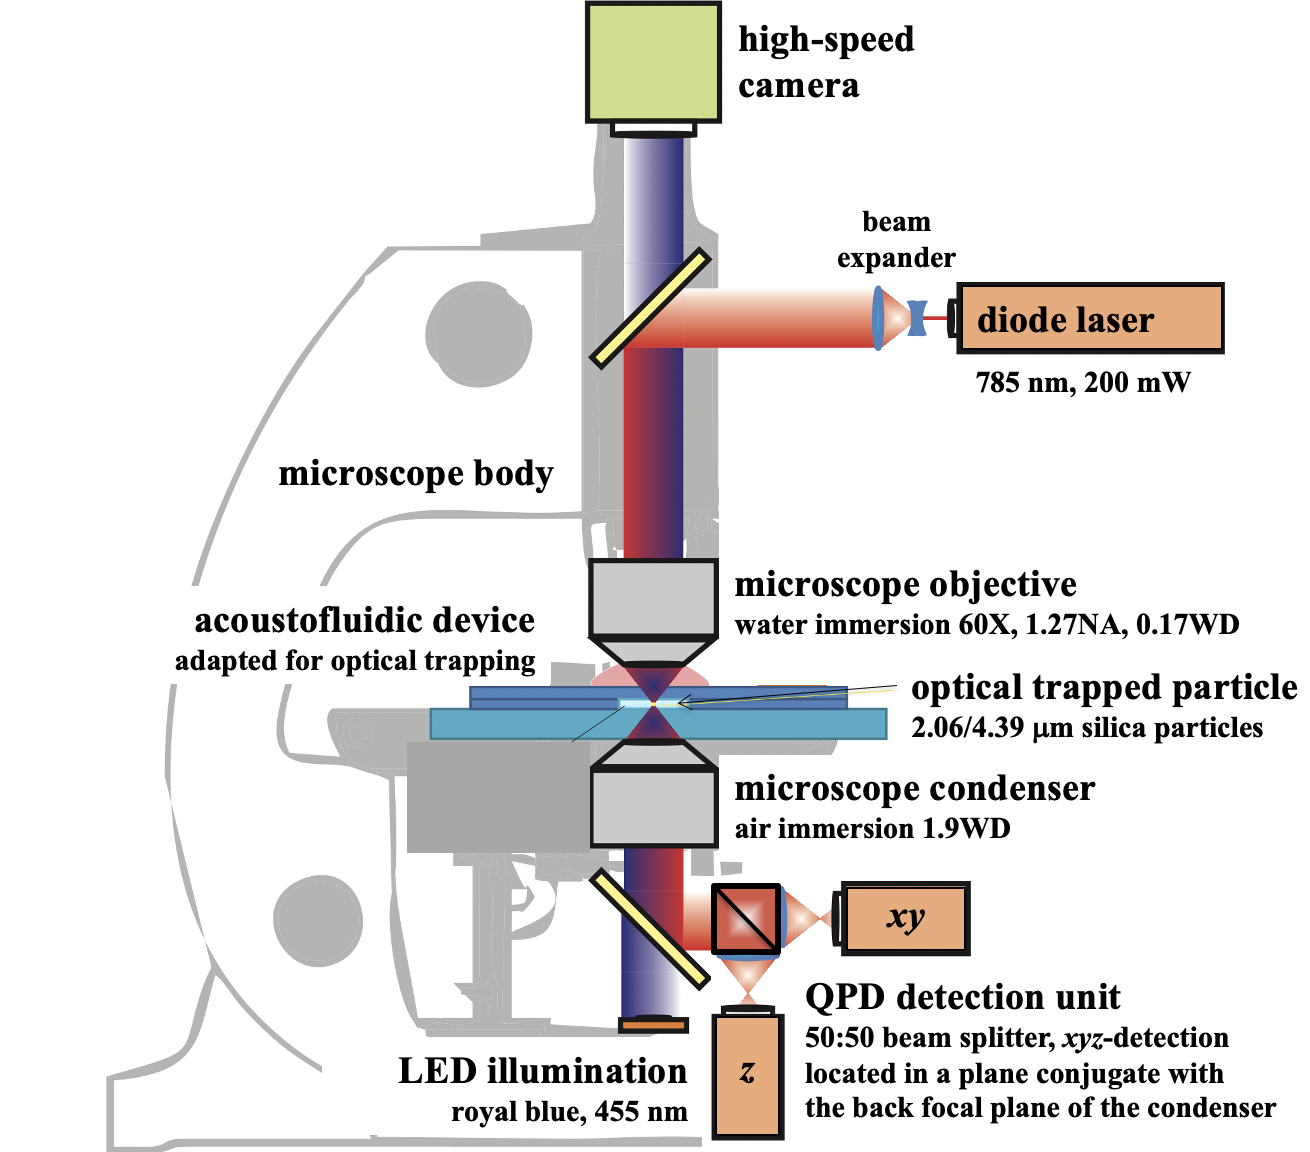
\includegraphics[width=84mm]{Fig2.png}
    \caption{The optical trap is based on a commercial upright microscope body.  
        The linear polarized laser light (\SI{785}{\nano\meter}) is aligned on 
        an optical table and coupled into the microscope. The microscope 
        objective forms the laser focus for trapping, and the condenser directs 
    the laser light to the detection unit, where QPDs are used for the analysis 
  of the particle displacements. An LED illuminates the sample and a high-speed 
camera is used for imaging.\label{fig:Fig2}}
\end{figure}%
%%%%%%%%%%%%%%%%%%%

The laser beam is projected onto a Quadrant Photo Detector (QPD) that is 
conjugated with the back focal plane of the condenser \cite{Bodensiek}. The 
QPD-$xy$ in \cref{fig:Fig2} is optimized to detect the $xy$-displacement of 
optically trapped particles. The laser spot size on the QPD-$xy$ is about 
\SI{2}{\mm} in diameter and the \SI{8}{\mm} diameter sensor measures 
displacements of the beam in the back focal plane. The QPD-$z$ measures the 
total laser intensity over its four quadrants which scales with the 
z-displacement of the particle inside its optical potential \cite{Dreyer}.

The analog data of the QPDs is anti-aliasing filtered at \SI{15}{\kilo\hertz} 
and is digitized by a data acquisition board (NI USB-6356, National Instruments, 
Austin, TX, US) with a sampling frequency of \SI{1}{\MS} (1 million samples per 
second). We recorded the Brownian motion of the particle within the optical trap 
for ten seconds and then performed a Fast Fourier Transform (FFT) on this signal 
to achieve a frequency resolution of $\Delta f=\SI{0.1}{\hertz}$. This spectrum 
is averaged over 10 cycles such that the calibration takes \SI{100}{\second}.  
The recorded signals are then further processed for calibration and force 
measurements in 3D with a self-written Matlab and LabVIEW (National Instruments, 
Austin, TX, US) routine.  Calibration of the position (\si{\meter\per\volt}) and 
force sensitivity (\si{\newton\per\meter}) was obtained via the Equipartition 
Theorem \cite{Svoboda,Vermeulen}. These calibrations are performed for the $x$-, 
$y$- and $z$-directions simultaneously. Due to the elongated shape of the focal 
spot in the $z$-direction, the optical trap stiffness $\kappa_z$ is 3 to 5 times 
weaker than the trapping stiffness in $x$- and $y$-direction. 

Here, a typical optical trapping stiffness for \SI{100}{\milli\watt} laser power 
and \SI{2.06}{\micro\meter} silica particles is 
\SI{2.9}{\femto\newton\per\micro\meter} in the $xy$-plane and 
\SI{1.1}{\femto\newton\per\micro\meter} in the $z$-direction. During the 
experiments it was ensured with the magnitude of the laser power that the 
displacements $u$ of the particles remained inside the valid regime of the trap 
calibration ($u<\sfrac{R}{2}$). The main counteracting force is the acoustic 
radiation force. With our Optical Trap setup we can stably trap particles 
between \SI{2}{\micro\meter} to \SI{10}{\micro\meter}. Larger particles tend to 
show unstable trapping in our setup.
% unstable trapping in our setup; smaller particles get closer to the used laser 
% wavelength ($\lambda = \SI{785}{\nano\meter}$) whereas our calibration method is 
% derived for $\lambda < R_{\text{particle}}$.

The spatial positioning of the optical trap in the $xy$-direction and 
$z$-direction was performed by a closed-loop motorized microscope stage (SCAN, 
Marzhauser, Wetzlar, Germany) and closed-loop piezo stage (PI, P-725.2CD, 
Karlsruhe, Germany), respectively. The statistic force repeatability of the 
optical trapping set-up was $\pm \SI{11}{\femto\newton}$ \cite{Lamprecht2016}, 
which includes positional drifts and eventual variations in temperature.

\subsection{Acoustofluidic Flow Cell\label{sec:VT-DeviceAndAcoustics}}

Within the optical trap, the working distance of the microscope objective 
(\SI{0.17}{\milli\meter}) and of the condenser (\SI{1.9}{\milli\meter}) limits 
the thickness of the flow cell.  Furthermore, the device has to be transparent 
for the laser wavelength $\lambda$ to permit optical trapping and detection (see 
\cref{fig:Fig2}). Therefore, a transparent glass device was built from a stack 
of standardized microscope coverslips (MENZEL GmbH, Braunschweig, Germany). It 
was designed to excite two individual standing waves in $x$- and $y$-direction 
separately, which provide the necessary conditions to rotate spherical 
\si{\micro\meter} particles. 

Similar as in \citeauthor{Lakamper} \cite{Lakamper}, a polyurethane spray glue 
(ITW, Cramolin Urethan, Muehlacker, Germany) was used for the fabrication of the 
micro-fluidic flow cells. Two square shaped coverslips of size (thickness, 
\numrange{0.13}{0.17} \si{\milli\meter}, and \SI{22x22}{\mm} large) were glued 
together and afterwards a \SI{4.0}{\milli\meter} wide cross-shaped fluid channel 
was diced into the center of one of the two coverslips. The remaining material 
of the diced coverslip was covered by another adhesive layer and glued onto a 
rectangular glass (thickness, \numrange{0.13}{0.17} \si{\milli\meter}, 
\SI{60}{\mm} long, \SI{22}{\mm} wide). The resulting stack of coverslips formed 
two crossed fluid channels in $x$- and $y$-direction with open ends (soft 
acoustic boundaries). The maximal distance of the fluid cavity depth plus the 
top cover thickness is $< \SI{270}{\micro\meter}$ as depicted in 
\cref{fig:Fig3}. An adapted phenolic paper with the size of a standard specimen 
slide ($l$, $w$, and $h$ = \numlist{75; 25; 1} \si{\mm}) holds the stacks of 
coverslips, so that the acoustic flow cell can be easily placed in the sample 
holder of the microscope stage.

%%%%%%%%%%%%%%%%%%%
\begin{figure}
    \centering
    \includegraphics[width=84mm]{Fig3.png}
    \caption{Stack of three coverslips form the device where the middle layer 
    includes two fluid channels (\SI{4.0x22}{\mm} with a depth of 
    \numrange{0.13}{0.17} \si{\milli\meter}, red boxes) in an orthogonal 
    arrangement. The two channels intersect and form a \SI{4.0x4.0}{\mm} crossed 
    chamber (black hatched area). Each piezo-electric transducer 
    \SI{4.0x2.0x0.5}{\mm} (PZ26, blue boxes) individually excites a direction.  
    The relative phase difference $\zeta$ of the excitation signals is freely 
    adjustable. The phenolic paper holds the stack and has the size of a 
    standard specimen slide for mounting.\label{fig:Fig3}}
\end{figure}
%%%%%%%%%%%%%%%%%%%

Two piezo-electric transducers (Ferroperm, Pz26, $l$, $w$, and $h$ = \numlist{4; 
2; 1} \si{\mm}, Kvistgaard, Denmark) were glued on the stack of coverslips with 
conductive glue (EPOXY Technology, H20E, Billerica, MA, USA) perpendicular to 
each channel in $x$- and $y$-direction. The distance between the center of the 
fluidic chamber and each transducer was \SI{7}{\mm}. This distance was set such, 
that the microscope objective stays clear from the transducers. The resulting 
thin design of the device ensured the usage of the optical trap and decoupled 
the standing wave modes in the channels ($x$ and $y$). This specific design 
enabled controlled excitation of standing wave modes in the directions of $x$ 
and $y$ as well as an individual control of the excitation phase $\zeta$ (see 
\cref{fig:Fig4}).

For our measurements we always used the same spatial position within the device.  
Hence, the rotation of the particles is always in the same direction for our 
experiments. However, \citeauthor{lamprecht2015} \cite{lamprecht2015} 
demonstrated how the rotation direction is dependent on the spatial location and 
the phase $\zeta$ of the two standing waves. In addition, in the supplemental 
material two videos are provided that show the change of rotation direction when 
changing these two parameters.

%%%%%%%%%%%%%%%%%%%
\begin{figure}
    \centering
    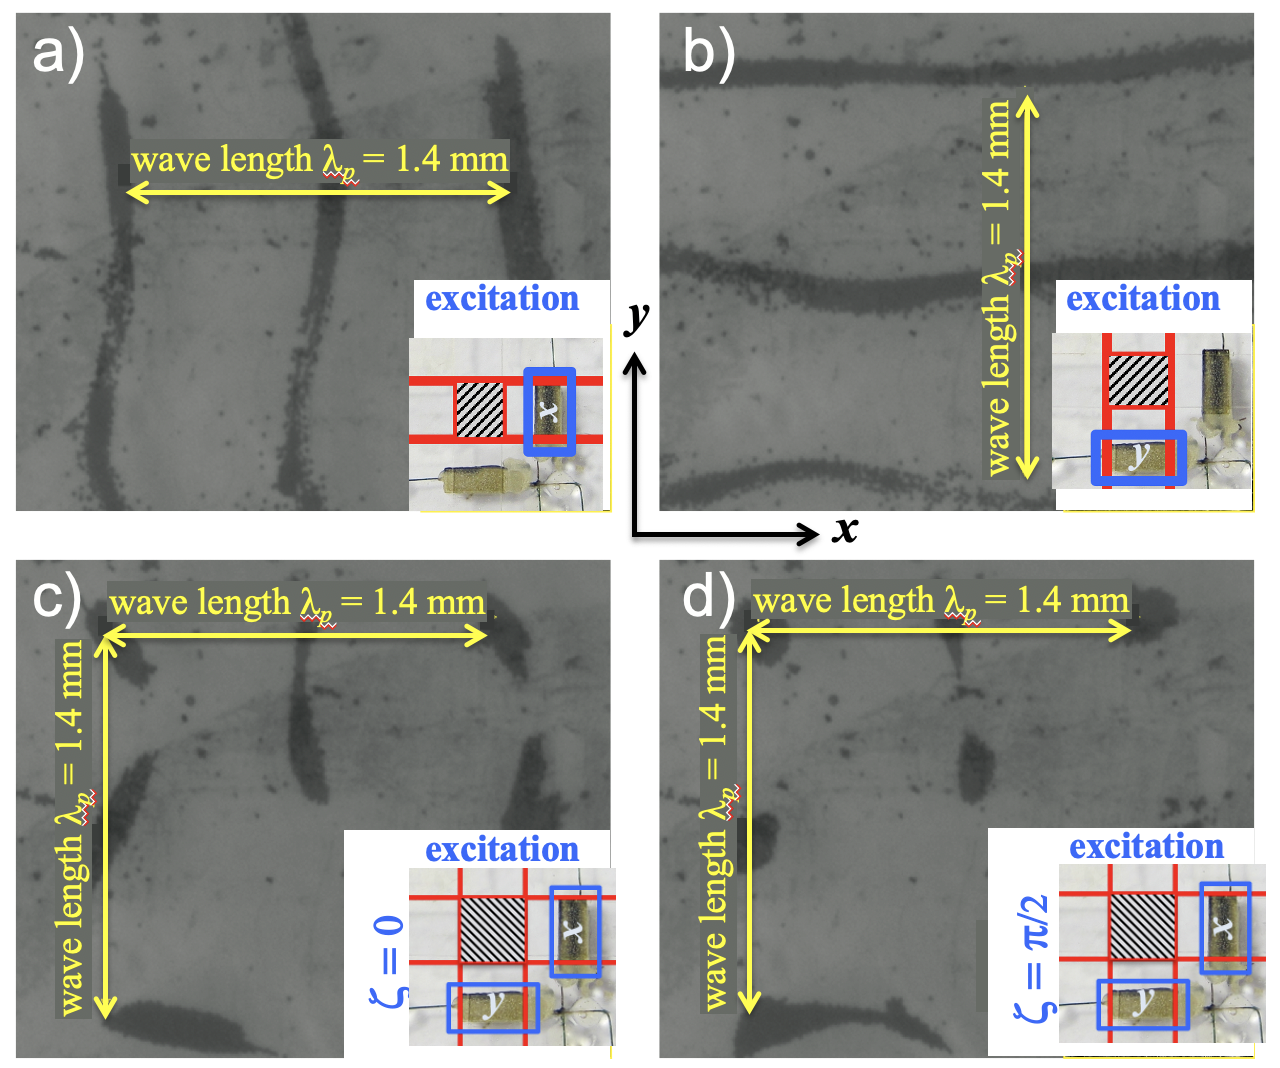
\includegraphics[width=84mm]{Fig4.png}
    \caption{The device is filled with a water/glycerol (70$\%$/30$\%$) mixture 
    containing \SI{4}{\micro\meter} copolymer particles (Duke Scientific 
    Cooperation, Palo Alto, CA, USA) and it has two identical modes in $x$- and 
    $y$-direction at \SI{1.043}{\mega\hertz}. a) and b) depict the isolated 
    modes at \SI{15}{\Vrms} for the $x$- and $y$-direction, respectively. The 
    resulting measured wavelength $\lambda_{P}$ was approximately 
    \SI{1.4}{\milli\meter} for both directions.\ c) and d) show the particle 
    pattern for the two orthogonal standing waves inside the crossed-fluid 
    chamber at $\zeta= 0$ and $\zeta= \frac{\pi}{2}$, respectively. These 
    observations confirm the assumption of a 2 dimensional orthogonal standing 
    wave field.\label{fig:Fig4}}
\end{figure}
%%%%%%%%%%%%%%%%%%%


\subsection{Particles \label{sec:VT-particles}}
For the visualization experiment in \cref{fig:Fig4} we used \SI{4}{\micro\meter} 
copolymer particles (Duke Scientific Cooperation, Palo Alto, CA, USA). For the 
optical trapping experiments with single particles we used silica particles 
because they are more precise in their dimensions compared to polystyrene 
particles. In addition, they have better interactions
with the acoustical field. Moreover, the results of \citeauthor{hahn2016} 
\cite{hahn2016} suggest that in the region of $R \approx \delta$ and ratios of 
$\sfrac{\rho_{\text{s}}}{\rho_{\text{f}}}$ between 2 and 15 result a greater 
magnitude of the acoustic viscous torque results. With the used fluid ($\rho_{f} 
= \SI{1.1}{\gram\per\cubic\centi\meter}$) and our silica particles ($\rho_{s} = 
\SI{2.0}{\gram\per\cubic\centi\meter}$) the ratio 
$\sfrac{\rho_{\text{s}}}{\rho_{\text{f}}} \approx 1.8$.

In order to validate the proposed power spectrum method two sets of validation 
experiments are explained in \cref{sec:VT-rotationDetectionValidation}. For those 
the \SI{4.39}{\micro\meter} particles were modified differently for each 
experiment. We use this size of particles since they are better visible when 
simultaneously measuring the rotation with a camera. There was the need to 
\emph{mark} the spherical \SI{4.39}{\micro\meter} silica particles because a 
reliable rotation measurement with the camera of unmarked spherical particles 
was not possible.

Two methods for marking were used. In both cases the rotation could be easily 
tracked by optical microscopy because the particle size of 
\SI{4.39}{\micro\meter} silica glass micro-spheres (Microparticles
GmbH, Berlin, Germany) is much larger than the optical resolution.
For the set of experiments, silica particles were deformed between two polished 
metal plates by applying a pressure of \SI{1}{\mega\pascal} to achieve a slight 
degree of non-sphericalness (see \cref{fig:Fig5}). For the second set, uncoated 
particles were distributed on a glass specimen slide (MENZEL GmbH, 
Menzel-Glaesser, Braunschweig, Germany) and coated by a Sputter coater (B7340 
Manual Sputter Coater, Van Loenen Instruments, Zaandam, Netherlands) with a gold 
coating (see \cref{fig:Fig6}). After coating, the particles were half-covered 
with a \SIrange{10}{20}{\nano\meter} thick gold layer at their surface 
orientated to the gold electrode. The coating affected the acoustic properties 
not substantially. The particles showed, i.e., same trapping and rotational 
behavior within the acoustical trap. Averted particle surfaces showed a thinner 
gold layer of about \SIrange{0}{10}{\nano\meter}.

\section{Experimental Procedure\label{sec:VT-experimentalProcedure}}

The observed time-averaged spatial off-set of the particles inside the optical 
trap is naturally zero, but the frequency content of the observed particle 
motion includes the thermal energy content of the particle as well as its 
rotational frequency. The angular frequency appears as an additional peak in the 
power spectrum of the rotating particle. In order to validate this detection 
method, particles with a rotational rate of less than \SI{1.66}{\hertz} 
(\SI{100}{\rpm}) were observed by a high-speed camera (HiSpec1 G2 Mono, Fastec, 
San Diego, USA) while also recording their power spectrum.  In the validation 
experiments the transparent device was filled with \SI{4.39}{\micro\meter} 
silica glass micro-spheres suspended in distilled water at a low concentration 
of a few particles per \si{\micro\liter}.  This low particle concentration does 
not effect the ratio $\tilde{\rho} = \sfrac{\rho_{\text{s}}}{\rho_{\text{f}}}$. 
The open channel ends were sealed with silicone oil to ensure a constant fluid 
volume during the measurements.

\subsection{Rotation Detection 
Validation\label{sec:VT-rotationDetectionValidation}}

Two sets of validation experiments were performed: (i) non-spherical particle 
rotation with slightly non-spherical particles; (ii) spherical particle rotation 
with gold covered particles for increased contrast in the video observation 
\cite{Lamprecht2013}. 

According to \citeauthor{Hahn2016} \cite{Hahn2016}, non-spherical objects can 
also be rotated due to the acoustic VT, but here effects of acoustic radiation 
torques may govern or influence their rotations \cite{Wang2012}. A slightly 
non-spherical \SI{4.39}{\micro\meter} silica particle (see \cref{fig:VT-Fig5}) was 
trapped in the optical potential well with \SI{100}{\milli\watt} laser power and 
moved to the reference position ($x,y,z = 0$) in the center of all three 
dimensions of the fluid chamber. The acoustic pressure field is formed by two 
orthogonal standing waves at the same excitation frequency of 
\SI{1090}{\kilo\hertz} and \SI{10.0}{\Vrms} amplitude. The particle was then 
optically moved to the closest resulting pressure node (intersection of two 
pressure nodal lines in $x$- and $y$-direction) with respect to the reference 
position. Positions of the pressure nodes were determined by a previous set of 
experiments.

The phase difference between the acoustic excitation directions $x$- and 
$y$-direction was set to $\zeta=\sfrac{\pi}{2}$, and the non-spherical particle 
rotated counter-clockwise with $\Omega = \SI{1.12}{\hertz}\,(\SI{67}{\rpm})$ 
(arithmetic mean of \SI{0.3}{\hertz} (\SI{18}{\rpm}) and \SI{1.6}{\hertz} 
(\SI{96}{\rpm}); see also \cref{fig:VT-Fig5}). At $\zeta=0$ the particle did not 
rotate because of the stable, non-varying acoustic potential.

%%%%%%%%%%%%%%%%%%%
\begin{figure}
    \centering
    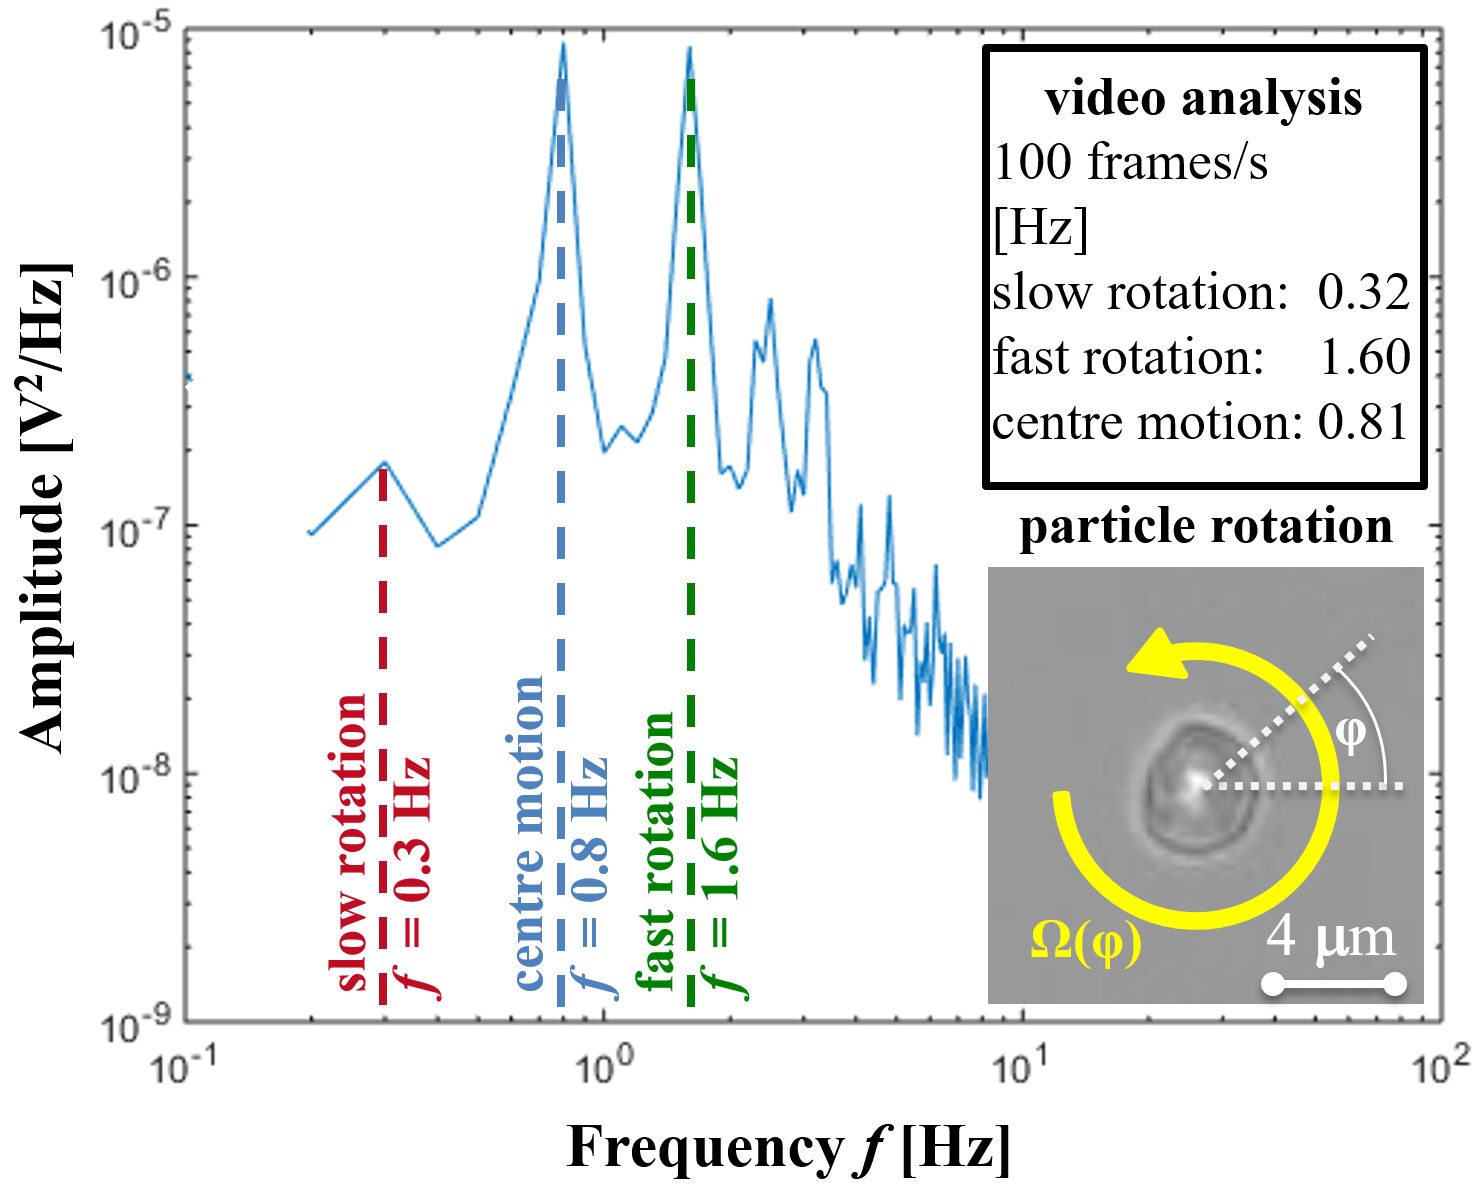
\includegraphics[width=100mm]{\relPath/10_Figures/Fig5.png}
    \caption{Power spectral density and results of the video analysis of a 
      counter-clockwise rotating non-spherical silica particle at 
      \SI{1090}{\kilo\hertz} and \SI{10.0}{\Vrms} with relative phase shift of 
      $\zeta= \sfrac{\pi}{2}$. The 10 times averaged power spectrum of the 
      $y$-signal of the detection unit (QPD) was recorded with a frequency 
      resolution of $\Delta f = \SI{0.1}{\hertz}$ and a sampling rate of 
      \SI{1}{\MS}. Three main peaks were observed at \numlist{0.3; 0.8; 1.6} 
      \si{\hertz}. The frequency peak at \SI{0.8}{\hertz} corresponds to a 
      relative $xy$-motion of the trapped particle, whereas the peaks at 
      \numlist{0.3; 1.6} \si{\hertz} (\numlist{18;96} \si{\rpm}) are related to 
      a non-constant angular rotation $\Omega(\varphi)$ of the particle. The 
      measured results are in correlation with the determined rotational rate by 
      the high-speed video analysis with a frame rate of \SI{100}{\fps}. See the 
      supplemental material for a optically trapped particle rotating 
      sequentially with two velocities due to its imperfect spherical 
  shape.\label{fig:VT-Fig5}}
\end{figure}%
%%%%%%%%%%%%%%%%%%%

In \cref{fig:VT-Fig5}, the average of 10 power spectral density plots is depicted, 
each obtained from a \SI{10}{\second} recording. The frequency resolution is 
$\Delta f=\SI{0.1}{\hertz}$. Three main peaks were observed in the power 
spectrum at \numlist{0.3; 0.8; 1.6} \si{\hertz}, which correlate with the 
frequencies detected by the contemporaneous video detection. We see these peaks 
on both QPDs for the $x-$ and $y$-direction. However for some of the latter 
rotational measurements, the $xy$-motion of the particle adds more peaks 
depending on the major axis of the acoustic displacement. All other peaks are 
related to multiple repetitions of these angular frequencies due to deviations 
of the spherical shape of the particle.  The peak at \SI{0.8}{\hertz} 
corresponds to a relative $xy$-motion of the particle, whereas the peaks at 
\numlist{0.3; 1.6} \si{\hertz} are related to angular frequencies of the 
non-constant rotation $\Omega(\varphi)$ of the particle. The existence of two 
frequency peaks is related to the influence of different acoustic pressures in 
$x$ and $y$-direction because the amplitude were not yet matched for this 
validation.  Hence, the acoustic radiation forces on the particle have different 
magnitudes in $x$ and $y$-direction. So, the distribution of acoustic radiation 
pressure on the particle changes during its rotation and leads to an additional 
orientation dependent acoustic radiation torque.  The influence of acoustic 
radiation forces on particle orientations is a well-known effect for small 
non-spherical particles with $r \ll \lambda$ \cite{Konig1891,Garbin2015}, but 
this experiment shows that this influence is also large enough to influence the 
rotation by the acoustic VT.  Particles with a larger degree of 
non-sphericalness did not even start to rotate in this set of experiments. This 
is in agreement with the predictions of \citeauthor{Hahn2016} \cite{Hahn2016}, 
that the acoustic VT decreases with a higher degree of elliptical shape of the 
particles. In contrast, the acoustic radiation torque increases and hinders a 
constant rotation of the particle, if the symmetry of the experimental acoustic 
potential at $\zeta= \sfrac{\pi}{2}$ is imperfect.

Previously, optical traps formed by a linearly polarized laser have been applied 
to rotate anisotropic particles \cite{GutirezMedina2010}. However, this torque 
is dependent on the orientation of the anisotropic particle with respect to the 
polarization plane of the laser. If the laser power is high enough, the 
acoustically induced rotation can be inhibited because the anisotropic particle 
is optically locked to the polarization plane. For perfectly spherical particles 
without any shape anisotropy this optical torque vanishes 
\cite{Manzo2006,Friese1998}. We did not observe influences of optical forces on 
the final rotational velocities of the spherical particles because the 
determined velocities in the experiments were independent of the applied laser 
power. For our validation experiments with deformed and gold coated particles we 
did not investigate further the influence of the linearly polarized laser on the 
particles. This indicates that the applied acoustic torque was greater in 
magnitude than the optical torque.

Also, the experiments that are presented afterward show that the particle 
rotation is dominated by the acoustic field. By moving the particle through the 
flow cell or by changing the phase of the excitation signal, the rotation can be 
stopped, started and reversed (see \cref{fig:VT-Fig8} and the video in the 
supplemental material).

A closer investigation was not possible in our current experimental set-up 
because particles sank due to gravity if the laser was turned off. Observed 
rotations near fluid boundaries (bottom plate) are governed by influences of 
near-boundary effects, e.g.\ higher viscous drag, different acoustic scattering 
and streaming which would complicate an investigation of low laser powers on the 
particle rotation.

The second set of validation experiments employed spherical particles with a 
thin gold layer to increase the contrast for the video observation 
\cite{Lamprecht2013}. The additional gold layer changed the optical properties of 
the particles and led to a different optical trapping behavior in the 
experiments. Most of the particles could not be trapped optically because the 
gold layer reflected the incident laser light (\SI{785}{\nano\meter}) and the 
resulting optical scattering forces pushed the particles away from the laser 
focus \cite{Zhou2020,Ashkin1992,Svoboda1994}. The particle needs to be 
transparent for the wavelength of the laser, in order to enable trapping. 
However, due to statistical variations of the coating process some particles 
were optically trappable, since just a small portion of the surface was coated.  
And hence, just a small portion of the incoming laser was reflected. One example 
of an optically trapped particle with a constant and stable rotation is shown in 
\cref{fig:VT-Fig6}. The brighter regions at the surface of the particle arise from 
the reflected laser light due to the partial gold coating.  These regions 
rotated with the optically trapped particle due to the acoustic VT.\@ The 
angular change of reflected light on the particle surface was then determined by 
the QPDs of the optical detection unit and increased the signal strength by a 
factor of 100 with respect to uncoated particles. The recorded power spectrum of 
the $x$- and $y$-signals included the information about the angular frequency of 
the rotating particle.

An example for a recorded power spectrum of a rotating gold-layered 
\SI{4.39}{\micro\meter} silica particle at an acoustic excitation frequency of 
\SI{1090}{\kilo\hertz} and amplitude of \SI{2.5}{\Vrms} with a relative phase 
shift of $\zeta= \sfrac{\pi}{2}$ is depicted in \cref{fig:VT-Fig6}. A clear peak 
can be seen at \SI{1.3}{\hertz}. The determined rotational rate of the particle 
by video observations was \SI{1.31}{\hertz} (\SI{78.6}{\rpm}), which correlates 
with the measured peak at \SI{1.3}{\hertz} (\SI{78.0}{\rpm}).  A further 
variation of the acoustic excitation parameters (amplitude and relative phase) 
shifted the peaks in frequency as predicted by 
\cref{eq:VT-Eq1,eq:VT-AcGovEqConti} (results are not shown) 
\cite{Lamprecht2013}.

%%%%%%%%%%%%%%%%%%%
\begin{figure}
    \centering
    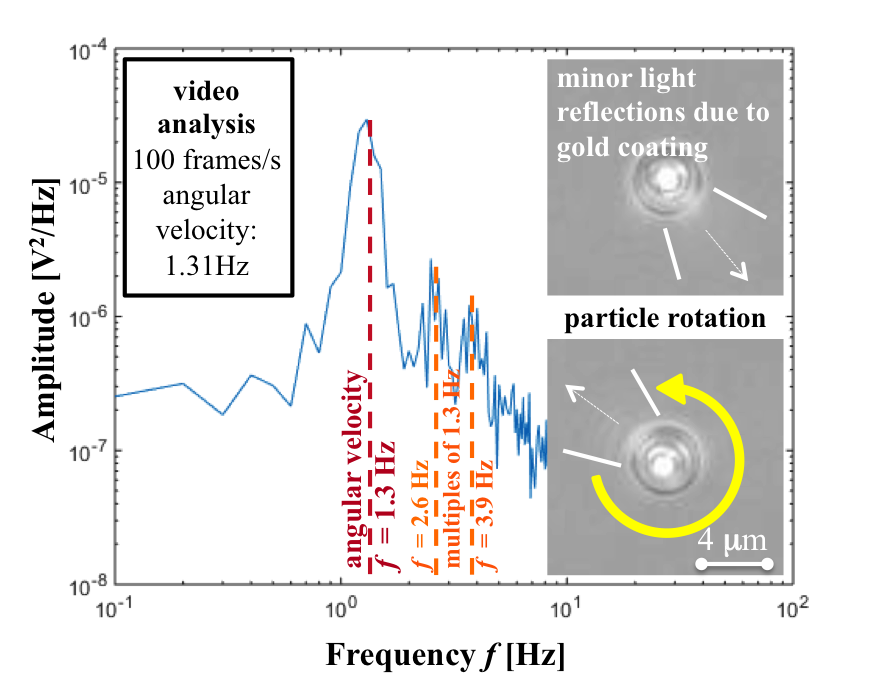
\includegraphics[width=100mm]{\relPath/10_Figures/Fig6.png}
    \caption{Power spectral density and results of the video analysis of a 
      counter-clockwise rotating gold-coated spherical \SI{4.39}{\micro\meter} 
      silica particle at \SI{1090}{\kilo\hertz} and \SI{2.5}{\Vrms} with 
      relative phase shift $\zeta= \sfrac{\pi}{2}$. The 10 times averaged power 
      spectrum of the $y$-signal of the detection unit (QPD) was recorded with a 
      frequency resolution of $\Delta f=\SI{0.1}{\hertz}$ and a sampling rate of 
      \SI{1}{\MS}. A clear peak at \SI{1.3}{\hertz} and two additional peaks at 
      \numlist{2.6; 3.9} \si{\hertz} were observed. The amplitudes of the 
      additional peaks were one order of magnitude smaller as the amplitude of 
      the peak at \SI{1.3}{\hertz}. The peak at \SI{1.3}{\hertz} correlates with 
  the determined rotational rate by the high-speed video analysis at a frame 
  rate of \SI{100}{\fps}.\label{fig:VT-Fig6}}
\end{figure}%
%%%%%%%%%%%%%%%%%%%

\subsection{Rotation of particles where $\normBdLayer \approx 
1$\label{sec:VT-rotationParticles}}

The determinations of the rotational rate with the power spectrum-method opened 
the possibility to measure fast rotations ($>\SI{25}{\hertz}$ (\SI{1500}{\rpm})) 
of particles with a radius $R$ about \SI{1}{\micro\meter}.  For such small 
particles the ratio of the thickness of the viscous boundary layer $\delta$ and 
the particle radius $R$ approaches 1 ($\normBdLayer \approx 1$) in the 
\si{\mega\hertz}-range (\SIrange{1}{10}{\mega\hertz}). The analytical formulas 
become invalid for the case that $\normBdLayer > \sfrac{1}{15}$ \cite{Hahn2016}.  
Particle rotations within the limit $\normBdLayer \approx 1$ were experimentally 
validated by an investigation of silica spheres with a \SI{2.06}{\micro\meter} 
(Microparticles GmbH, Berlin, Germany) diameter resuspended with a 
water/glycerol (70$\%$/30$\%$) mixture.  The viscosity $\mu_f$ of the aqueous 
glycerol solution was \SI{0.06}{\pascal\second} \cite{Jerome1968} with a 
determined density of \SI{1.1}{\gram\per\centi\meter\cubed} (dense knife, DMA 
35N, Anton Paar GmbH, Graz, Austria) and increased the thickness of the viscous 
boundary layer to approximately \SI{1.33}{\micro\meter} at an excitation 
frequency of \SI{1043}{\kilo\hertz} ($\lambda \approx \SI{1.4}{\mm}$). The 
normalized viscous boundary layer is therefore $\normBdLayer \approx 1.30$.

The optical trapping set-up was originally designed to measure the acoustic 
force and pressure amplitudes inside micro-fluidic channels and cavities 
\cite{Lakaemper2015,Lamprecht2016}. The same procedure was used here to measure 
the local acoustic pressure amplitudes inside the fluid chamber of the 
transparent micro-device. An accurate prediction of the acoustic pressure 
amplitudes $A_{X}$ and $A_{Y}$ of the two orthogonal standing waves was 
important to determine the strength of the acoustic VT by observing the 
steady-state rotational rate $\finalOmega$ of rotating particles.

Therefore, the local acoustic pressure amplitudes $A_{X}$ and $A_{Y}$ were 
individually measured in $x$- and $y$-direction by exciting only one transducer 
of the corresponding $x$- or $y$-direction, respectively. We measured the 
acoustic forces in all three dimensions ($x$, $y$, $z$) acting on the 
\SI{2.06}{\micro\meter}-particle inside the optical trapping potential. The 
spatial measurement range was $\pm \SI{0.55}{mm}$ in the $x$- and $y$-direction.  
The point $(\SI{0.21}{\mm}, \SI{0.22}{\mm})$, measured relatively to the middle 
of the fluid chamber, corresponded to the spatial position where a pressure 
nodal line in $x$- and $y$-direction overlapped.

The maximal force amplitudes at \SI{1043}{\kilo\hertz} were 
\SIrange{-96}{+25}{\femto\newton} for the $x$-direction and 
\SIrange{-32}{28}{\femto\newton} for the $y$-direction. The peak-to-peak value 
of the determined forces in $y$-direction was about two times weaker than in 
$x$-direction. This factor of 2 was used to calibrate the piezoelectric 
excitation amplitude to reach equal acoustic pressure amplitudes in both 
excitation directions.

The excitation amplitude $U_{el}$ is proportional with the acoustic pressure 
amplitude $A_{x,y}$ ($U_{el} \propto A_{x,y}$), whereas the acoustic radiation 
force $F_{ac}$ has a quadratic dependency of the acoustic pressure amplitudes 
$A_{x,y}$ ($F_{ac} \propto A_{x,y}^2$) \cite{Barnkob2010}. Therefore, the 
excitation amplitude of the piezoelectric transducer in $y$-direction was 
increased by a factor of $\sqrt{2}$ for all further investigations. The acoustic 
pressure amplitude $p_{a}$ was calculated via
%%%%%%%%%%%%%%%%%%%
\begin{equation}
\label{eq:VT-PressurePredictions}
\begin{split}
p_{a}^{2} &= \frac{F}{\pi\,R^{3}\,\kappa_{0}\,\Phi(f_{1},f_{2})} 
\frac{1}{k\,\sin(2k\,x)}\\
&= \frac{F}{\pi\,R^{3}\,\kappa_{0}\,\Phi(f_{1},f_{2})} 
\frac{\lambda_{\text{p}}}{2\pi\,\sin(x\,\sfrac{4\pi}{\lambda_{\text{p}}})}
\end{split}
\end{equation}
%%%%%%%%%%%%%%%%%%%
where a 1-dimensional standing plane wave is assumed \cite{Settnes2012a}. $F$ is 
the force measured with the optical trap, $\lambda_{\text{p}}$ the wavelength of 
the pressure field, $k = \sfrac{2\pi}{\lambda_{\text{p}}}$ the wavenumber, $R$ 
the radius of the spherical particle, $\kappa_{0}$ the compressibility of the 
fluid, $\Phi(f_{1},f_{2})$ the so-called acoustic contrast factor, and 
$\sin(kx)$ the spatial dependency of the standing wave.  Since the force was 
measured at the force maximum $\sin(2\,kx)$ is set to $\sin(\sfrac{\pi}{2}) = 
1$. In addition, because of the value for the normalized viscous boundary layer 
$\normBdLayer \approx 1$, the corrected dipole factor  
$f_{2}(\tilde{\rho},\normBdLayer)$ of \citeauthor{Settnes2012} 
\cite{Settnes2012} was utilized. With this, the determined acoustic pressure 
amplitude for the standing wave in $x$-direction was \SI{245}{\kilo\pascal} for 
the measured acoustic forces and wavelength if an influence of acoustic 
streaming was neglected. 

After the calibration of the excitation amplitudes and the acoustic pressures of 
both acoustofluidic channels the acoustic VT was quantitatively investigated 
inside the fluid chamber. One \SI{2.06}{\micro\meter} silica particle was 
optically trapped and moved in $x$-direction inside the wave field of two 
orthogonal standing waves, while measuring its power spectrum at specified 
measurements points. The location of one specific pressure nodal line for an one 
dimensional standing wave in $x$- and $y$-direction at \SI{1043}{\kilo\hertz} 
was determined at $x=\SI{0.21}{\mm}$ and $y=\SI{0.22}{\mm}$, respectively. These 
nodal lines formed a local pressure node at their intersection if the acoustic 
excitation was shifted in phase with $\zeta = \sfrac{\pi}{2}$. There, the 
acoustic VT had its maximum value. Therefore, a measurement line in 
$x$-direction was defined between $x=0.20\pm0.55~\si{\milli\meter}$ at constant 
$y=\SI{0.22}{\milli\meter}$.

The particle exerted a counter-clockwise rotation at the local pressure node due 
to the acoustic VT at \SI{1043}{\kilo\hertz} with \SI{10.0}{\Vrms} and 
\SI{14.2}{\Vrms} excitation amplitude in $x$- and $y$-direction, respectively.

The detection of the angular frequency in a recorded power spectrum was not 
trivial for those small and spherical silica particles due to their low 
signal-to-noise ratios. Additionally, the power spectrum was disturbed by added 
frequencies of the acoustic excitation set-up; namely, an additional peak at 
\SI{100}{\hertz} originating from the voltage supply and \SI{170}{\hertz} from 
the amplifier itself.  Therefore, all measurements were repeated with a 
ten-times lower excitation amplitudes in $x$- and $y$-direction to calibrate the 
power spectrum measurements due to unknown influences of the environment and 
attached set-ups. An initialization of particle rotations was not observed at 
these low excitation amplitudes. A peak detection algorithm (implemented in 
MatLab) used the calibration measurement to eliminate disturbances on the 
determined power spectrum of a locally rotating particle due to VT.\@

\Cref{fig:VT-Fig8} depicts the power spectrum of a rotating particle with a clear 
peak at a frequency of \SI{165}{\hertz}. The particle was located at the 
relative location (-0.075, 0.220) \si{\mm} and its rotation was initialized at 
\SI{1043}{\kilo\hertz} with an excitation amplitude of \SI{10.0}{\Vrms} and 
\SI{14.2}{\Vrms} in $x$- and $y$-direction, respectively.  An appearance of 
additional peaks at a multiple of the angular frequency was not monitored by the 
peak-detection algorithm, likely because the amplitude of these peaks was below 
the noise floor. Their signal strength was expected to be one order of 
magnitude smaller (see \cref{fig:VT-Fig5,fig:VT-Fig6}).  The detection 
algorithm had a threshold value of 3 (signal-to-noise ratio) for indicating 
peaks in determined power spectrum.  \cref{fig:VT-Fig8}b depicts the 
corresponding calibration power spectrum of \cref{fig:VT-Fig8}a.

\Cref{fig:VT-Fig10} depicts the peaks detected by the peak-detection algorithm. 
Each point represents a separate rotational rate measurement. Interestingly, the 
strength of the angular frequency peaks was proportional to Brownian noise with 
$\sfrac{1}{f^2}$. These peaks are due to the particle rotations at positions 
within the spatial range of $x=0.21\pm\SI{0.55}{\mm}$ and $y=\SI{0.22}{\mm}$.  
The spatial dependency and formation of these peaks were in correlation with 
\cref{eq:VT-Eq1} and the maximal frequency $f$ of a peak in the power spectrum was 
\SI{229}{\hertz} ($ \finalOmega = \SI{13.8e3}{\rpm} $). The quantitative 
analysis revealed that maximal rotation appeared at $x=\SI{0.16}{\mm}$ (pressure 
node) and the resulting acoustic wavelength in $x$-direction was \SI{1.9}{\mm}.  
A one-dimensional wave in water at $f=\SI{1043}{\kilo\hertz}$ predicts an 
acoustic wavelength of $\lambda = \sfrac{c}{f} \approx \SI{1.4}{\mm}$ (compare 
\cref{fig:VT-Fig4}). The difference in wavelength from \cref{fig:VT-Fig4} 
($\lambda \approx \SI{1.4}{\mm} $) to the fitted value of $\lambda \approx 
\SI{1.9}{\mm} $ may be related to an off-set in orientation of the 
3-dimensional wavenumber $|\vb{k}|^{2} = k^{2}_{x} + k^{2}_{y} + k^{2}_{z}$ in 
the optical trapping set-up. Eigenfrequencies and their acoustic fields are 
influenced by the optical trapping set-up due to the additional interface 
between the acoustofluidic device and the water-immersion objective 
\cite{Lamprecht2016}.  \Cref{fig:VT-Fig4} was observed with a standard 
microscope lens that did not need to have an immersion oil layer on top of the 
device.

%%%%%%%%%%%%%%%%%%%
\begin{figure}
    \centering
    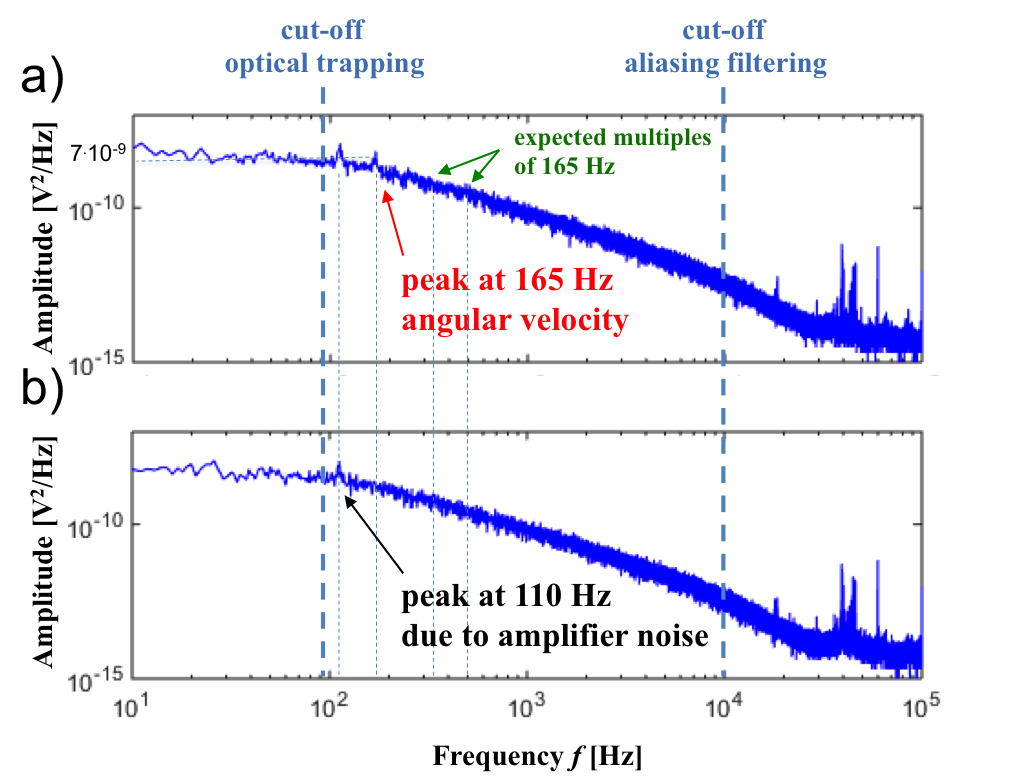
\includegraphics[width=100mm]{\relPath/10_Figures/Fig9.png}
    \caption{a) Measured power spectrum of an optically trapped 
    \SI{2.06}{\micro\meter} particle that rotated counter-clockwise due to the 
    acoustic VT at \SI{1043}{\kilo\hertz} with \SI{10.0}{\Vrms} and 
    \SI{14.2}{\Vrms} excitation amplitude in $x$- and $y$-direction, 
    respectively. The particle was located at (-0.075, 0.220) \si{\mm}. The 
    spectrum of the $x$-signal (QPD) was recorded and 10 times averaged with a 
    frequency resolution of $\Delta f=\SI{1}{\hertz}$ and a sampling rate of 
    \SI{1}{\MS}. A clear signal peak due to particle rotation at 
  \SI{165}{\hertz} was observed with a signal-to-noise ratio of about 5. The 
signal peak at \SI{110}{\hertz} is related to influences of the acoustic 
excitation set-up.\ b) Control measurement of a non-rotating optically trapped 
\SI{2.06}{\micro\meter} particle under acoustic excitation at 
\SI{1043}{\kilo\hertz} with \SI{1}{\Vrms} and \SI{1.42}{\Vrms} excitation 
amplitude in $x$- and $y$-direction, respectively. A particle rotation was not 
initialized at these low excitation amplitudes and these recorded power spectrum 
of non-rotating \si{\micro\meter} particles were used to identify the peaks not 
related to particle rotation power spectrum due to influences of the environment 
and the acoustic excitation set-up. The peak at \SI{110}{\hertz} is related to 
amplifier noise and vanished when the acoustic excitation set-up was turned off 
\cite{Lamprecht2016}.\label{fig:VT-Fig8}}
\end{figure}
%%%%%%%%%%%%%%%%%%%

%%%%%%%%%%%%%%%%%%%
\tikzsetnextfilename{VT_results}
\begin{figure}[tb]
  \centering
  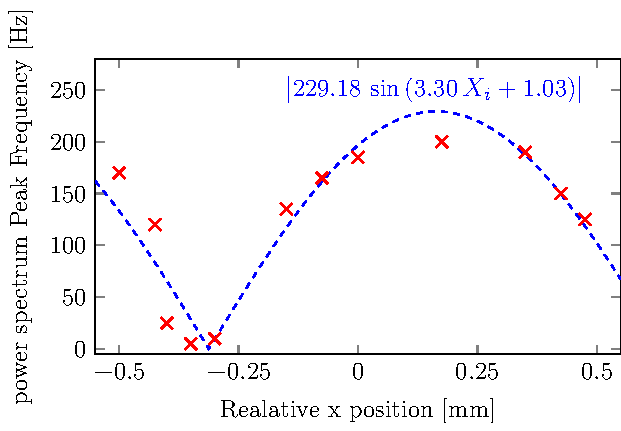
\includegraphics[]{External/VT_results.pdf}
    % \begin{tikzpicture}
    %     \begin{axis}
    %         [scale only axis,
    %         width = 89mm,
    %         height = 5cm,
    %         xtick = {-0.5,-0.25,0,0.25,0.5},
    %         xmin = -0.55, xmax = 0.55,
    %         ymax = 280, ymin = -5,
    %         xlabel = {Realative x position [\si{\mm}]},
    %         ylabel = {power spectrum Peak Frequency [\si{\hertz}]}]

    %         \addplot[red,thick,mark size=4pt,only marks,mark=x] table[x=y, 
    %         y=f,col sep=comma] {\relPath/40_Fitting/datapoints.dat};

    %         \addplot[thick,blue,dashed] table[x=y, y=f,col sep=comma] 
    %         {\relPath/40_Fitting/datapointsFit.dat};

    %         \node[blue,above] at (axis cs: 0.16,229) 
    %         {$\left|229.18\,\sin\left(3.30\,X_{i} + 1.03 \right)\right|$};

    %     \end{axis}
    % \end{tikzpicture}
    \caption{Spatial dependency of frequency peaks (red) due to the acoustic VT 
      from the power spectrum-method. Multiple power spectra of a 
      \SI{2.06}{\micro\meter} silica particle were recorded at specific 
      measurement points in $x$-direction at $x=\SI{0.21}{\mm}\pm\SI{0.5}{\mm}$ 
      and $y=\SI{0.22}{\mm}$. The acoustic field formed two orthogonal standing 
      waves in $x$- and $y$-direction at \SI{1043}{\kilo\hertz} with a relative 
      phase shift of $\zeta =\frac{\pi}{2}$. The determined frequency peaks were 
      fitted to the equation $\left|c_{1}\,\sin(c_2\,X_i + c_3)\right|$ (dashed 
      blue).  The resulting maximal frequency $f$  from the fit was 
      \SI{229}{\hertz} ($ \finalOmega = \SI{13.8e3}{\rpm}$) and the determined 
      acoustic wave in $x$-direction $\lambda_{X}=\sfrac{2\pi}{c_2}$ was 
    \SI{1.90}{\mm}. The pressure nodal point with maximal rotational rate was 
  determined at $x=\SI{0.16}{\mm}$, whereas zero VT was determined at 
$x=\SI{-0.31}{\mm}$ (pressure anti-node).\label{fig:VT-Fig10}}
\end{figure}
%%%%%%%%%%%%%%%%%%%

\section{Conclusion\label{sec:VT-conclusion}}

The combination of an optical trap and a transparent VT device opened the 
possibility to measure the VT independently of the acoustic radiation force. The 
power spectrum analysis provided the quantitative information about the angular 
frequency $\Omega$. Unwanted effects related to close proximities of walls near 
the rotating particle and influences of oscillating micro gas bubbles were 
avoided.  The optically levitated particle ensured a largely unaffected rotation 
due to the acoustic VT.\@ 

Moving the stage of the optical set-up changed the rotation direction of a 
trapped and rotated particle between two neighboring pressure nodes because of 
the acoustic VT \cite{Lamprecht2015} (see the supplemental material for a 
particle rotation in different directions depending on the spatial location 
inside the wave field).  These kinds of experiments were so far unattainable in 
a continuous manner and for unstable acoustic particle positions (positive 
acoustic contrast factor) of zero VT.\@

The validation experiments showed that the detected additional peaks in the 
measured power spectrum are directly related to the rotational rate of the 
particle rotation. The detected signals had peaks at multiples of this peak 
frequency.  However, for transparent silica particles with an almost perfectly 
spherical shape the amplitudes of the multiples were too small to overcome the 
signal-to-noise-ratio. The high-speed video analysis is limited by the camera's 
frame rate. In contrast, the detection bandwidth of the optical trap easily 
spans tens of \si{\kilo\hertz}. As already mentioned, optical trapping has some 
unique advantages to investigate the acoustic VT: 1) Allows to probe almost  any 
spatial position within the acoustofluidic device. 2) Measures rotational 
frequencies up to multiple \si{\kilo\hertz}. 3) Works with conventional, non 
coated, spherical particles. 4) Frequencies are directly visible in the data (no 
need for post processing of video data).

In order to calculate the theoretical rotational rate $\finalOmega$ of the 
particle, the local acoustic pressure amplitude needs to be known in advance.  
Because of that, a local acoustic pressure amplitude analysis was carried out 
before the rotation detection experiments. Depending on the calculation 
approach, different results are obtained for the rotational rate. The analytical 
calculation for the final rotational rate $\finalOmega$ (see \cref{eq:VT-Eq1}) 
\cite{Lamprecht2015, Busse1981, Rudnick1977, Wang1989} with a dynamic fluid viscosity of 
$\mu_{f} = \SI{0.06}{\pascal\second}$ led to rates between 
\SIrange{613}{811}{\hertz} (\SIrange{36.8e3}{48.7e3}{\rpm}). The numerical 
calculations of \citeauthor{Hahn2016} \cite{Hahn2016} yield a final rotational 
rate for a \SI{2.06}{\micro\meter} silica particle with $\normBdLayer=1.30$ of 
\SIrange{208}{277}{\hertz} (\SIrange{12.5e3}{16.6e3}{\rpm}) at room temperature 
(\SI{25}{\celsius}).  The first value for the rotational rate corresponds each 
time to the theoretical wavelength of $\lambda \approx \SI{1.4}{\mm}$ (see 
\cref{fig:VT-Fig4}) and acoustic pressure amplitude $p_{a}\left(\lambda\right) = 
\SI{245}{\kilo\pascal} $; the latter to the measured $\lambda \approx 
\SI{1.9}{\mm}$ (see \cref{fig:VT-Fig10}) and $p_{a}\left(\lambda\right) = 
\SI{282}{\kilo\pascal} $. The disagreement between our experiments and 
\cref{eq:VT-Eq1} is regarding the equilibrium state for the final rotational rate 
$\finalOmega$. The spatial dependency of \cref{eq:VT-Eq1} ($\cos\left(k\,X\right), 
\cos\left( k\,Y \right)$) agrees with our experiments.

In contrast to that, the power spectrum-method estimates the steady-state 
rotational rate $\finalOmega$ to \SI{229}{\hertz} (\SI{13.8e3}{\rpm}). This 
value is very close to the numerically obtained values (about 10$\%$ higher for 
$\lambda \approx \SI{1.4}{\mm}$ or 17$\%$ lower for $\lambda \approx 
\SI{1.9}{\mm}$).  These deviations can be in part explained by a decrease of 
the fluid viscosity due to laser-induced heating (up to \SI{2}{\kelvin}) in 
close proximity of the laser focus \cite{Peterman2003}. Since the measured force 
of our trap scales with $\sqrt{\mu}$ and the viscosity variation around 
\SI{25}{\celsius} is relatively small, the temperature induced measurement 
errors are about 2\%.  This slightly changes the acoustic pressure amplitudes 
with respect to the calibrated pressure of \SI{245}{\kilo\pascal} ($\lambda 
\approx \SI{1.4}{\mm}$) or \SI{282}{\kilo\pascal} ($\lambda \approx 
\SI{1.9}{\mm}$) because the investigated pressure node was located slightly off 
the calibration lines.  Also, the in oil immersed lens of the optical trap 
changes the theoretical (pure) 1-dimensional acoustic field to a 3-dimensional.

The experiment clearly showed that the analytical calculations of 
\citeauthor{Lamprecht2015,Busse1981, Rudnick1977, Wang1989} \cite{Lamprecht2015, Busse1981, 
Rudnick1977, Wang1989}  overestimate the rotational velocities at ratios $\normBdLayer 
\approx 1$. Furthermore, the complexity and spatially varying torques on 
\si{\micro\meter} particles were measured, whereas the simulations are limited 
to the ideal case of plane-standing waves and incompressible particles in an 
infinitely large fluid domain. 

A further application of the acoustic torque analysis with an optical trap could 
be the experimental determination of the influence of the particle density on 
the acoustic VT.\@ Particles with the same density can show different rotational 
directions at a fixed point in the acoustic field, if the ratio $\normBdLayer$ 
changes \cite{Hahn2016}.

Optical torques on double refracting quartz particles is a possible tool to 
directly measure acoustic torques \cite{La2004}. The laser power of such 
modulated optical traps could be used to calibrate acoustic torques on trapped 
particles at equilibriums where the optical torque counteracts the acoustic 
torque. 

% \vspace*{7mm}

% A.L and C.G. contributed equally to this work.



% \appendix
% \begin{appendix}
% %\iffalse %Beginn langer Kommentar
\chapter[Appendix]{Supplemental to Chapter 5\label{ch:app-pulsing}}

% \end{appendix}
% \cleardoublepage

% \renewcommand{\bibname}{References} %Rename chapter to References
\addcontentsline{toc}{chapter}{References} %add references to Outline
% \bibliographystyle{siam}
% \bibliography{All}
\printbibliography


\setlength{\parindent}{0mm} %Abschnitt-Einzug auf 0 setzen
\renewcommand{\\}{\newline} %damit wird wieder \\ \\ möglich für doppelte Zeilenabstände


% \chapter*{List of Publications}
\markboth{List of Publications}{List of Publications}                     % heading
\addcontentsline{toc}{chapter}{List of Publications}          % list in table 


\makeatletter
\DeclareCiteCommand{\fullcite}
  {\defcounter{maxnames}{\blx@maxbibnames}%
    \usebibmacro{prenote}}
  {\usedriver
     {\DeclareNameAlias{sortname}{default}}
     {\thefield{entrytype}}}
  {\multicitedelim}
  {\usebibmacro{postnote}}
\DeclareCiteCommand{\footfullcite}[\mkbibfootnote]
  {\defcounter{maxnames}{\blx@maxbibnames}%
    \usebibmacro{prenote}}
  {\usedriver
     {\DeclareNameAlias{sortname}{default}}
     {\thefield{entrytype}}}
  {\multicitedelim}
  {\usebibmacro{postnote}}
\makeatother

%as first author}
\section*{Publications in Peer-Reviewed Scientific Journals}
\begin{itemize}
  \item \fullcite{Lamprecht2021}\footnote{A.L. and C.G. shared first author}
  \item \fullcite{Goering2021}
  \item \fullcite{Goering2022}
  \item \fullcite{Fankhauser2022}\footnote{J.F. and C.G. shared first author}
\end{itemize}


\section*{Oral Presentations at International Conferences}
C. Goering, A. Lamprecht, I.A.T. Schaap, and J. Dual.  \emph{"Direct 
Measurement of Small Spherical Particle Rotation driven by the Acoustic Viscous 
Torque"} Acoustics Virtually Everywhere, 07-11 December 2020, Virtual 
Conference.\\
  \\
C. Goering and J. Dual.\emph{"Measuring the temporal difference in build up 
between the acoustic radiation force and acoustic streaming with an optical 
tweezer."} Acoustofluidics, 26-27 August 2021, Virtual Conference.\\

% \thispagestyle{empty}

\makeatletter
\newcommand\tabfill[1]{%
  \dimen@\linewidth
  \advance\dimen@\@totalleftmargin
  \advance\dimen@-\dimen\@curtab
  \parbox[t]\dimen@{#1\ifhmode\strut\fi}%
}
\makeatother

\begin{floatingfigure}{4.5cm} %Abstand vom rechten Rand (formerly 3.5)
\centerline{ 
\includegraphics[trim={50mm 30mm 50mm 30mm}, clip, width=35mm]{SECTION/Portrait.png}} 
% \label{portrait}
\end{floatingfigure}

\noindent\textbf{ \\ \underline{Christoph} Ludwig Georg Ananda Goering} \\
\begin{flushleft}
\noindent  Born on 17$^\mathrm{th}$ of August 1991 in Augsburg, Germany \\
\end{flushleft}

\vspace{2.8cm} \noindent
\textbf{Education}                                        \\
\vspace{-0.5cm} \noindent


\begin{tabbing}
  \hspace{25mm} \=   \kill


2018--2022 \> \tabfill{PhD student in Prof. J. Dual's group, Institute of 
Mechanical Systems, Swiss Federal Institute of Technology (ETH) Zurich, 
Switzerland}\\
2015--2017 \> \tabfill{M.Sc. in mechanical engineering at the Technical 
University of Munich (TUM), Germany.}\\
2011--2014 \> \tabfill{B.Eng. in \emph{Maschinenbau -- Konstruktion und 
Entwicklung} at Dualen Hochschule Baden-Württemberg (DHBW), Ravensburg, 
Germany.}\\
2002--2011 \> \tabfill{Gymnasium bei St. Stephan, Augsburg; graduation with the 
German Abitur.}\\
\end{tabbing}

\vspace{-0.5cm} \noindent
\textbf{Professional experience}\\
\vspace{-0.8cm} \noindent
\begin{tabbing}
  \hspace{25mm} \=   \kill
  2018--2022 \> \tabfill{PhD Student at ETH, Zurich, Switzerland.}\\
  2015--2017 \> \tabfill{Werksstudent at BMW AG, Munich, Germany.}\\
  2011--2014 \> \tabfill{Dualer Student at Zeppelin Systems GmbH, 
  Friedrichshafen, Germany.}\\
  2011--2017 \> \tabfill{Auxiliary staff at MABRIS, Augsburg, Germany.}\\
\end{tabbing}

\vspace{-0.5cm} \noindent
\textbf{Extra curricular activities}\\
\vspace{-0.8cm} \noindent
\begin{tabbing}
  \hspace{25mm} \=   \kill
  2012--2015 \> \tabfill{Member of Global Formula Racing (GFR); winner of 
  multiple events overall in the Formula Student.}\\
  1991-- \> \tabfill{Being outdoors.}\\

\end{tabbing}


\end{document}
